\begin{frame}[t]{Intrusion Detection}
  \vspace{2em}
  \begin{block}{Intrusion Detection System (IDS)}
    IDSs monitor the behavior of a system to detect malicious activities.
  \end{block}

  \begin{figure}
    \centering
    \includegraphics<2>[width=.75\textwidth]{figures/intro/ids.pdf}
    \includegraphics<3>[width=.75\textwidth]{figures/intro/ids-us.pdf}
  \end{figure}
\end{frame}


\begin{frame}{Machine Learning for Intrusion Detection}

  \begin{itemize}
    \item Various types of algorithms: \alert<2>{supervised}, unsupervised, semi-supervised, reinforcement learning, \textit{etc}.
    \item Great performance with Deep Learning (DL) (on public datasets at least).
  \end{itemize}

  \pause
  \begin{columns}
    \begin{column}{0.5\textwidth}
        \textbf{Challenges:}
        \begin{itemize}
          \item not enough labelled data;
          \item risk of local bias or skewed data distribution;
          \item inefficient against new attacks, especially \alert{supervised} approaches.
        \end{itemize}
    \end{column}

    \begin{column}{0.5\textwidth}
      \begin{figure}
        \centering
        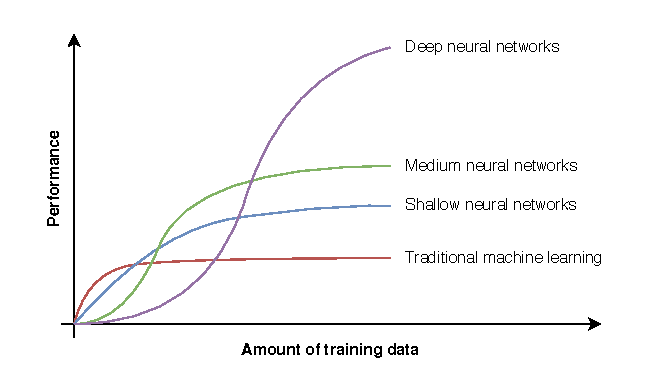
\includegraphics[width=\linewidth]{figures/intro/ml-perf}
      \end{figure}
    \end{column}
  \end{columns}
\end{frame}

\begin{frame}{Data Sharing}
% TODO:
% pas assez de données, faisons un pot commun !
% oui mais non :
% - confidentialité des données 
% - confiance dans le point de collecte
% - confiance dnas le processus d'apprentissage
% - pas de modèle de detection sans serveur
\begin{columns}
  \begin{column}{0.5\textwidth}
    \centering
    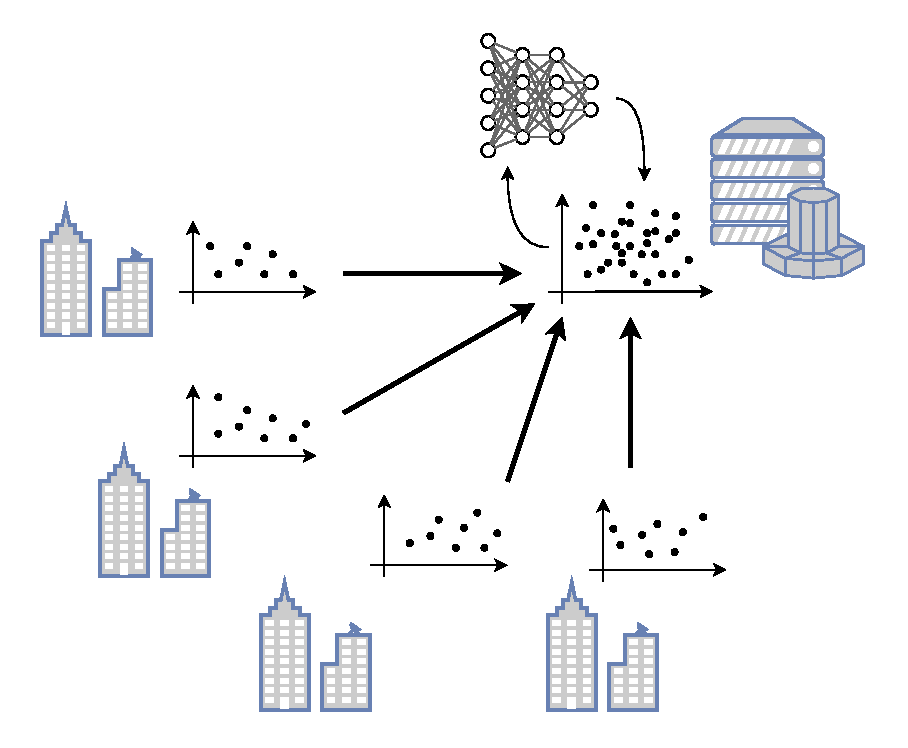
\includegraphics[width=\linewidth]{figures/intro/collab.pdf}
  \end{column}
  \begin{column}{0.5\textwidth}
    \textbf{Let's pool our data!}\pause{} \textbf{Although\dots}
    \begin{itemize}
      \item Privacy concerns.
      \item Lack of trust in the data holder.
      \item Lack of trust in the learning process.
      \item Lack of incentives.
      \item \dots
    \end{itemize}
  \end{column}
\end{columns}
\end{frame}


\begin{frame}{Scaling Intrusion Detection}

  \textbf{Federated Learning (FL)}
  
  \begin{itemize}[<+->]
    \item Novel-\emph{ish} distributed ML paradigm (Google, 2017)~\autocite{mcmahan_Communicationefficientlearningdeep_2017}.
    \item Distributed clients can train a common model without sharing their training data.
    \item \alert{Privacy-preserving}: high level of abstraction for the shared models preventing data leakage.
  \end{itemize}

  \fcitefootnote{mcmahan_Communicationefficientlearningdeep_2017}
\end{frame}


\begin{frame}{FL Fundamentals}
  \vspace{-1em}
  \begin{figure}
    \centering
    \foreach \i in {1,...,7} {%
      \includegraphics<\i>[width=.75\linewidth]{./figures/intro/fl/\i.pdf}%
    }
    \caption{Typical FL workflow, applied to NIDSs.}
  \end{figure}
\end{frame}


\begin{frame}{FL for NIDSs}

  \textbf{Benefits}
  \begin{itemize}[<+->]
    \item Virtually extended dataset with Horizontal FL.
    \begin{itemize}[<1->]
      \item Better generalization.
      \item Reduced risk of overfitting or local bias.
    \end{itemize}
    

    \item Effectively share knowledge (\eg, on specific classes, instances) between participants
    \begin{itemize}[<1->]
      \item Share the knowledge about a new attack~\autocite{lavaur_icdcs_demo_2024};
      \item Improve the characterization of specific devices; \dots
    \end{itemize}

    \only<2>{\fcitefootnote{lavaur_icdcs_demo_2024}}

  \end{itemize}
\end{frame}


\begin{frame}{Case Study}
  \bigskip
  \textbf{Collaborative Intrusion Detection between Distributed Organizations}
  \begin{itemize}
    \item Each organization has its own NIDS and monitors an information system.
    \item They want to improve their detection capabilities.
    \item Share knowledge about new attacks or specific devices.
  \end{itemize}
  \bigskip
  \pause
  \begin{figure}
    \centering
    \makebox[\textwidth][c]{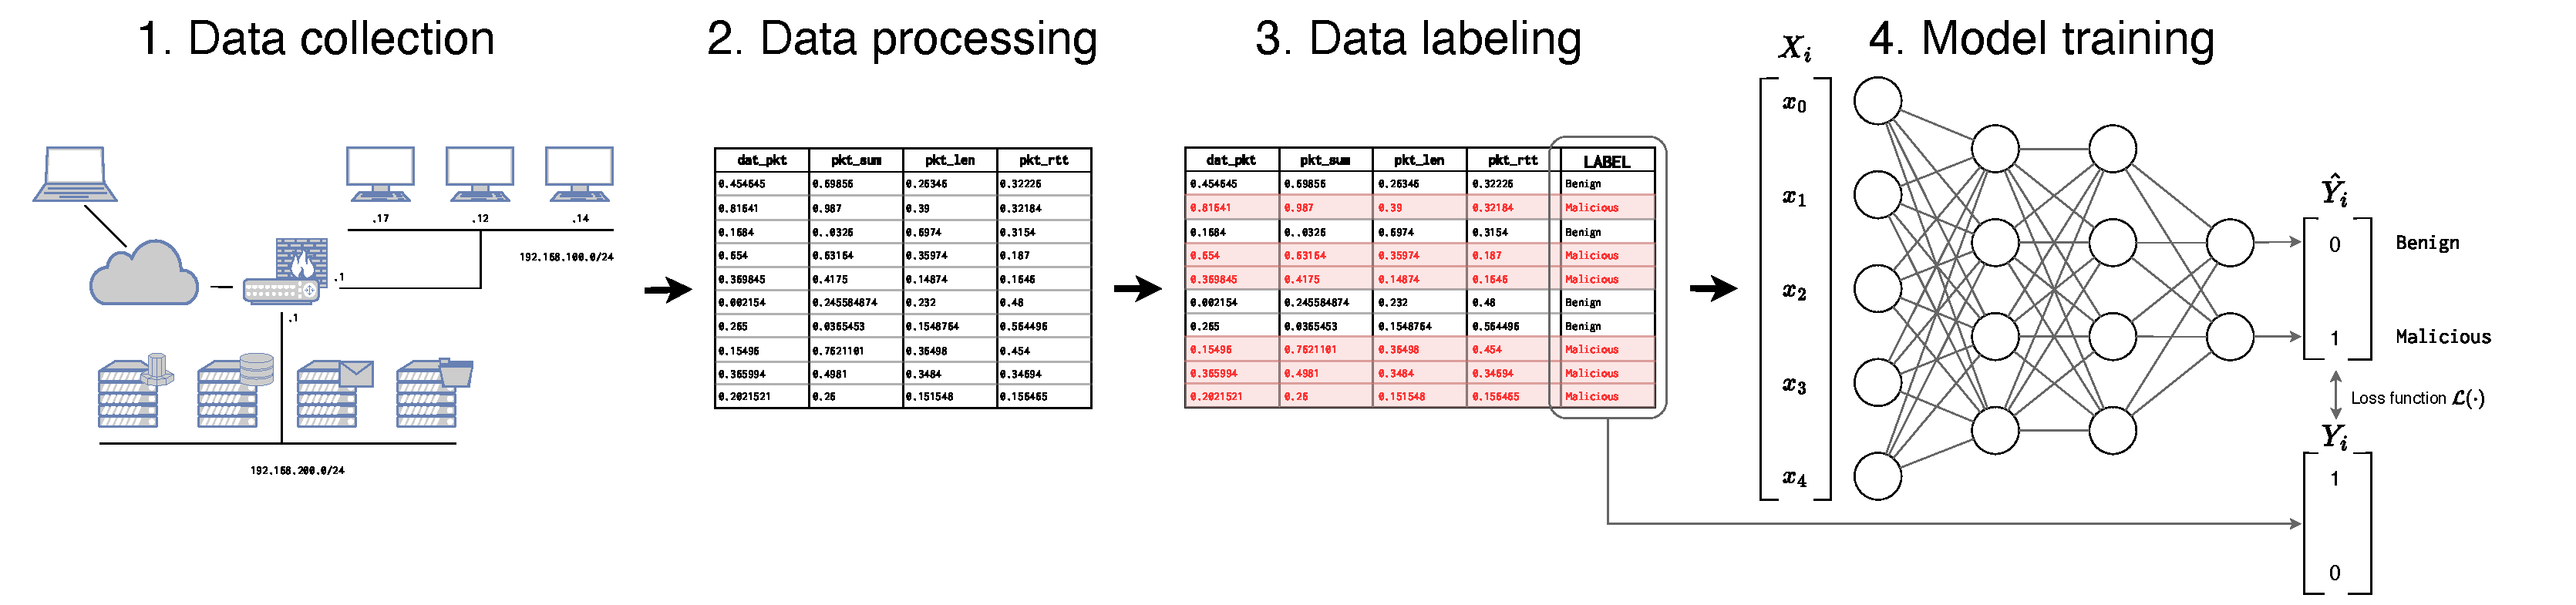
\includegraphics[width=.9\textwidth]{figures/intro/mlp-workflow.pdf}}
    \caption{Typical workflow for ML-based NIDSs.}
  \end{figure}
\end{frame}


\begin{frame}{Case Study -- Generalization}
  \textbf{A cross-silo use case}~\cite{kairouz_AdvancesOpenProblems_2021}:
  \begin{itemize}
    \item few clients (\ie, 10--100);
    \item consequent amount of data, high heterogeneity;
    \item high availability, significant computing resources.
  \end{itemize}
\end{frame}


\begin{frame}{State of the Art}
  
  \begin{columns}
    \begin{column}{.45\textwidth}
      % \textbf{Systematic Literature Review (SLR)}~\autocite{lavaur_tnsm_2022}
      % \begin{itemize}
      %   \item Booming topic over the last 4--5 years.
      %   \item Very heterogeneous venues and communities.
      % \end{itemize}

      \textbf{Challenges from the Literature}~\autocite{lavaur_tnsm_2022}
      \begin{itemize}[<+->]
        \item \emph{Functionality}: \chqual[5-]{performance}, \chhetero[5-]{heterogeneity}, \chtransfer[5-]{transferability}, self-defense, and self-healing.
        \item \emph{Deployment}: \chunknown[5-]{adaptability} and \chdecent[5-]{scalability}.
        \item \emph{Security and reliability}: \chpoison[5-]{security}, privacy, \chpoison[5-]{trust}, and reputation.
        \item \emph{Experimentation}: evaluation.
      \end{itemize}
    \end{column}
    \begin{column}{.55\textwidth}
      \only<4-5>{%
        \begin{figure}
          \centering
          \resizebox{\linewidth}{!}{%% Creator: Matplotlib, PGF backend
%%
%% To include the figure in your LaTeX document, write
%%   \input{<filename>.pgf}
%%
%% Make sure the required packages are loaded in your preamble
%%   \usepackage{pgf}
%%
%% Also ensure that all the required font packages are loaded; for instance,
%% the lmodern package is sometimes necessary when using math font.
%%   \usepackage{lmodern}
%%
%% Figures using additional raster images can only be included by \input if
%% they are in the same directory as the main LaTeX file. For loading figures
%% from other directories you can use the `import` package
%%   \usepackage{import}
%%
%% and then include the figures with
%%   \import{<path to file>}{<filename>.pgf}
%%
%% Matplotlib used the following preamble
%%   \def\mathdefault#1{#1}
%%   \everymath=\expandafter{\the\everymath\displaystyle}
%%   
%%   \usepackage{fontspec}
%%   \makeatletter\@ifpackageloaded{underscore}{}{\usepackage[strings]{underscore}}\makeatother
%%
\begingroup%
\makeatletter%
\begin{pgfpicture}%
\pgfpathrectangle{\pgfpointorigin}{\pgfqpoint{3.140876in}{1.985768in}}%
\pgfusepath{use as bounding box, clip}%
\begin{pgfscope}%
\pgfsetbuttcap%
\pgfsetmiterjoin%
\definecolor{currentfill}{rgb}{1.000000,1.000000,1.000000}%
\pgfsetfillcolor{currentfill}%
\pgfsetlinewidth{0.000000pt}%
\definecolor{currentstroke}{rgb}{1.000000,1.000000,1.000000}%
\pgfsetstrokecolor{currentstroke}%
\pgfsetdash{}{0pt}%
\pgfpathmoveto{\pgfqpoint{0.000000in}{0.000000in}}%
\pgfpathlineto{\pgfqpoint{3.140876in}{0.000000in}}%
\pgfpathlineto{\pgfqpoint{3.140876in}{1.985768in}}%
\pgfpathlineto{\pgfqpoint{0.000000in}{1.985768in}}%
\pgfpathlineto{\pgfqpoint{0.000000in}{0.000000in}}%
\pgfpathclose%
\pgfusepath{fill}%
\end{pgfscope}%
\begin{pgfscope}%
\pgfsetbuttcap%
\pgfsetmiterjoin%
\definecolor{currentfill}{rgb}{1.000000,1.000000,1.000000}%
\pgfsetfillcolor{currentfill}%
\pgfsetlinewidth{0.000000pt}%
\definecolor{currentstroke}{rgb}{0.000000,0.000000,0.000000}%
\pgfsetstrokecolor{currentstroke}%
\pgfsetstrokeopacity{0.000000}%
\pgfsetdash{}{0pt}%
\pgfpathmoveto{\pgfqpoint{0.374222in}{0.433222in}}%
\pgfpathlineto{\pgfqpoint{1.568043in}{0.433222in}}%
\pgfpathlineto{\pgfqpoint{1.568043in}{1.885768in}}%
\pgfpathlineto{\pgfqpoint{0.374222in}{1.885768in}}%
\pgfpathlineto{\pgfqpoint{0.374222in}{0.433222in}}%
\pgfpathclose%
\pgfusepath{fill}%
\end{pgfscope}%
\begin{pgfscope}%
\pgfpathrectangle{\pgfqpoint{0.374222in}{0.433222in}}{\pgfqpoint{1.193820in}{1.452545in}}%
\pgfusepath{clip}%
\pgfsetbuttcap%
\pgfsetmiterjoin%
\definecolor{currentfill}{rgb}{0.121569,0.466667,0.705882}%
\pgfsetfillcolor{currentfill}%
\pgfsetlinewidth{0.000000pt}%
\definecolor{currentstroke}{rgb}{0.000000,0.000000,0.000000}%
\pgfsetstrokecolor{currentstroke}%
\pgfsetstrokeopacity{0.000000}%
\pgfsetdash{}{0pt}%
\pgfpathmoveto{\pgfqpoint{0.391277in}{0.433222in}}%
\pgfpathlineto{\pgfqpoint{0.527713in}{0.433222in}}%
\pgfpathlineto{\pgfqpoint{0.527713in}{0.433222in}}%
\pgfpathlineto{\pgfqpoint{0.391277in}{0.433222in}}%
\pgfpathlineto{\pgfqpoint{0.391277in}{0.433222in}}%
\pgfpathclose%
\pgfusepath{fill}%
\end{pgfscope}%
\begin{pgfscope}%
\pgfpathrectangle{\pgfqpoint{0.374222in}{0.433222in}}{\pgfqpoint{1.193820in}{1.452545in}}%
\pgfusepath{clip}%
\pgfsetbuttcap%
\pgfsetmiterjoin%
\definecolor{currentfill}{rgb}{0.121569,0.466667,0.705882}%
\pgfsetfillcolor{currentfill}%
\pgfsetlinewidth{0.000000pt}%
\definecolor{currentstroke}{rgb}{0.000000,0.000000,0.000000}%
\pgfsetstrokecolor{currentstroke}%
\pgfsetstrokeopacity{0.000000}%
\pgfsetdash{}{0pt}%
\pgfpathmoveto{\pgfqpoint{0.561823in}{0.433222in}}%
\pgfpathlineto{\pgfqpoint{0.698259in}{0.433222in}}%
\pgfpathlineto{\pgfqpoint{0.698259in}{0.433222in}}%
\pgfpathlineto{\pgfqpoint{0.561823in}{0.433222in}}%
\pgfpathlineto{\pgfqpoint{0.561823in}{0.433222in}}%
\pgfpathclose%
\pgfusepath{fill}%
\end{pgfscope}%
\begin{pgfscope}%
\pgfpathrectangle{\pgfqpoint{0.374222in}{0.433222in}}{\pgfqpoint{1.193820in}{1.452545in}}%
\pgfusepath{clip}%
\pgfsetbuttcap%
\pgfsetmiterjoin%
\definecolor{currentfill}{rgb}{0.121569,0.466667,0.705882}%
\pgfsetfillcolor{currentfill}%
\pgfsetlinewidth{0.000000pt}%
\definecolor{currentstroke}{rgb}{0.000000,0.000000,0.000000}%
\pgfsetstrokecolor{currentstroke}%
\pgfsetstrokeopacity{0.000000}%
\pgfsetdash{}{0pt}%
\pgfpathmoveto{\pgfqpoint{0.732368in}{0.433222in}}%
\pgfpathlineto{\pgfqpoint{0.868805in}{0.433222in}}%
\pgfpathlineto{\pgfqpoint{0.868805in}{0.433222in}}%
\pgfpathlineto{\pgfqpoint{0.732368in}{0.433222in}}%
\pgfpathlineto{\pgfqpoint{0.732368in}{0.433222in}}%
\pgfpathclose%
\pgfusepath{fill}%
\end{pgfscope}%
\begin{pgfscope}%
\pgfpathrectangle{\pgfqpoint{0.374222in}{0.433222in}}{\pgfqpoint{1.193820in}{1.452545in}}%
\pgfusepath{clip}%
\pgfsetbuttcap%
\pgfsetmiterjoin%
\definecolor{currentfill}{rgb}{0.121569,0.466667,0.705882}%
\pgfsetfillcolor{currentfill}%
\pgfsetlinewidth{0.000000pt}%
\definecolor{currentstroke}{rgb}{0.000000,0.000000,0.000000}%
\pgfsetstrokecolor{currentstroke}%
\pgfsetstrokeopacity{0.000000}%
\pgfsetdash{}{0pt}%
\pgfpathmoveto{\pgfqpoint{0.902914in}{0.433222in}}%
\pgfpathlineto{\pgfqpoint{1.039351in}{0.433222in}}%
\pgfpathlineto{\pgfqpoint{1.039351in}{0.433222in}}%
\pgfpathlineto{\pgfqpoint{0.902914in}{0.433222in}}%
\pgfpathlineto{\pgfqpoint{0.902914in}{0.433222in}}%
\pgfpathclose%
\pgfusepath{fill}%
\end{pgfscope}%
\begin{pgfscope}%
\pgfpathrectangle{\pgfqpoint{0.374222in}{0.433222in}}{\pgfqpoint{1.193820in}{1.452545in}}%
\pgfusepath{clip}%
\pgfsetbuttcap%
\pgfsetmiterjoin%
\definecolor{currentfill}{rgb}{0.121569,0.466667,0.705882}%
\pgfsetfillcolor{currentfill}%
\pgfsetlinewidth{0.000000pt}%
\definecolor{currentstroke}{rgb}{0.000000,0.000000,0.000000}%
\pgfsetstrokecolor{currentstroke}%
\pgfsetstrokeopacity{0.000000}%
\pgfsetdash{}{0pt}%
\pgfpathmoveto{\pgfqpoint{1.073460in}{0.433222in}}%
\pgfpathlineto{\pgfqpoint{1.209897in}{0.433222in}}%
\pgfpathlineto{\pgfqpoint{1.209897in}{0.462043in}}%
\pgfpathlineto{\pgfqpoint{1.073460in}{0.462043in}}%
\pgfpathlineto{\pgfqpoint{1.073460in}{0.433222in}}%
\pgfpathclose%
\pgfusepath{fill}%
\end{pgfscope}%
\begin{pgfscope}%
\pgfpathrectangle{\pgfqpoint{0.374222in}{0.433222in}}{\pgfqpoint{1.193820in}{1.452545in}}%
\pgfusepath{clip}%
\pgfsetbuttcap%
\pgfsetmiterjoin%
\definecolor{currentfill}{rgb}{0.121569,0.466667,0.705882}%
\pgfsetfillcolor{currentfill}%
\pgfsetlinewidth{0.000000pt}%
\definecolor{currentstroke}{rgb}{0.000000,0.000000,0.000000}%
\pgfsetstrokecolor{currentstroke}%
\pgfsetstrokeopacity{0.000000}%
\pgfsetdash{}{0pt}%
\pgfpathmoveto{\pgfqpoint{1.244006in}{0.433222in}}%
\pgfpathlineto{\pgfqpoint{1.380442in}{0.433222in}}%
\pgfpathlineto{\pgfqpoint{1.380442in}{0.480116in}}%
\pgfpathlineto{\pgfqpoint{1.244006in}{0.480116in}}%
\pgfpathlineto{\pgfqpoint{1.244006in}{0.433222in}}%
\pgfpathclose%
\pgfusepath{fill}%
\end{pgfscope}%
\begin{pgfscope}%
\pgfpathrectangle{\pgfqpoint{0.374222in}{0.433222in}}{\pgfqpoint{1.193820in}{1.452545in}}%
\pgfusepath{clip}%
\pgfsetbuttcap%
\pgfsetmiterjoin%
\definecolor{currentfill}{rgb}{0.121569,0.466667,0.705882}%
\pgfsetfillcolor{currentfill}%
\pgfsetlinewidth{0.000000pt}%
\definecolor{currentstroke}{rgb}{0.000000,0.000000,0.000000}%
\pgfsetstrokecolor{currentstroke}%
\pgfsetstrokeopacity{0.000000}%
\pgfsetdash{}{0pt}%
\pgfpathmoveto{\pgfqpoint{1.414551in}{0.433222in}}%
\pgfpathlineto{\pgfqpoint{1.550988in}{0.433222in}}%
\pgfpathlineto{\pgfqpoint{1.550988in}{0.548504in}}%
\pgfpathlineto{\pgfqpoint{1.414551in}{0.548504in}}%
\pgfpathlineto{\pgfqpoint{1.414551in}{0.433222in}}%
\pgfpathclose%
\pgfusepath{fill}%
\end{pgfscope}%
\begin{pgfscope}%
\pgfpathrectangle{\pgfqpoint{0.374222in}{0.433222in}}{\pgfqpoint{1.193820in}{1.452545in}}%
\pgfusepath{clip}%
\pgfsetbuttcap%
\pgfsetmiterjoin%
\definecolor{currentfill}{rgb}{1.000000,0.498039,0.054902}%
\pgfsetfillcolor{currentfill}%
\pgfsetlinewidth{0.000000pt}%
\definecolor{currentstroke}{rgb}{0.000000,0.000000,0.000000}%
\pgfsetstrokecolor{currentstroke}%
\pgfsetstrokeopacity{0.000000}%
\pgfsetdash{}{0pt}%
\pgfpathmoveto{\pgfqpoint{0.391277in}{0.433222in}}%
\pgfpathlineto{\pgfqpoint{0.527713in}{0.433222in}}%
\pgfpathlineto{\pgfqpoint{0.527713in}{0.433222in}}%
\pgfpathlineto{\pgfqpoint{0.391277in}{0.433222in}}%
\pgfpathlineto{\pgfqpoint{0.391277in}{0.433222in}}%
\pgfpathclose%
\pgfusepath{fill}%
\end{pgfscope}%
\begin{pgfscope}%
\pgfpathrectangle{\pgfqpoint{0.374222in}{0.433222in}}{\pgfqpoint{1.193820in}{1.452545in}}%
\pgfusepath{clip}%
\pgfsetbuttcap%
\pgfsetmiterjoin%
\definecolor{currentfill}{rgb}{1.000000,0.498039,0.054902}%
\pgfsetfillcolor{currentfill}%
\pgfsetlinewidth{0.000000pt}%
\definecolor{currentstroke}{rgb}{0.000000,0.000000,0.000000}%
\pgfsetstrokecolor{currentstroke}%
\pgfsetstrokeopacity{0.000000}%
\pgfsetdash{}{0pt}%
\pgfpathmoveto{\pgfqpoint{0.561823in}{0.433222in}}%
\pgfpathlineto{\pgfqpoint{0.698259in}{0.433222in}}%
\pgfpathlineto{\pgfqpoint{0.698259in}{0.709898in}}%
\pgfpathlineto{\pgfqpoint{0.561823in}{0.709898in}}%
\pgfpathlineto{\pgfqpoint{0.561823in}{0.433222in}}%
\pgfpathclose%
\pgfusepath{fill}%
\end{pgfscope}%
\begin{pgfscope}%
\pgfpathrectangle{\pgfqpoint{0.374222in}{0.433222in}}{\pgfqpoint{1.193820in}{1.452545in}}%
\pgfusepath{clip}%
\pgfsetbuttcap%
\pgfsetmiterjoin%
\definecolor{currentfill}{rgb}{1.000000,0.498039,0.054902}%
\pgfsetfillcolor{currentfill}%
\pgfsetlinewidth{0.000000pt}%
\definecolor{currentstroke}{rgb}{0.000000,0.000000,0.000000}%
\pgfsetstrokecolor{currentstroke}%
\pgfsetstrokeopacity{0.000000}%
\pgfsetdash{}{0pt}%
\pgfpathmoveto{\pgfqpoint{0.732368in}{0.433222in}}%
\pgfpathlineto{\pgfqpoint{0.868805in}{0.433222in}}%
\pgfpathlineto{\pgfqpoint{0.868805in}{0.433222in}}%
\pgfpathlineto{\pgfqpoint{0.732368in}{0.433222in}}%
\pgfpathlineto{\pgfqpoint{0.732368in}{0.433222in}}%
\pgfpathclose%
\pgfusepath{fill}%
\end{pgfscope}%
\begin{pgfscope}%
\pgfpathrectangle{\pgfqpoint{0.374222in}{0.433222in}}{\pgfqpoint{1.193820in}{1.452545in}}%
\pgfusepath{clip}%
\pgfsetbuttcap%
\pgfsetmiterjoin%
\definecolor{currentfill}{rgb}{1.000000,0.498039,0.054902}%
\pgfsetfillcolor{currentfill}%
\pgfsetlinewidth{0.000000pt}%
\definecolor{currentstroke}{rgb}{0.000000,0.000000,0.000000}%
\pgfsetstrokecolor{currentstroke}%
\pgfsetstrokeopacity{0.000000}%
\pgfsetdash{}{0pt}%
\pgfpathmoveto{\pgfqpoint{0.902914in}{0.433222in}}%
\pgfpathlineto{\pgfqpoint{1.039351in}{0.433222in}}%
\pgfpathlineto{\pgfqpoint{1.039351in}{0.433222in}}%
\pgfpathlineto{\pgfqpoint{0.902914in}{0.433222in}}%
\pgfpathlineto{\pgfqpoint{0.902914in}{0.433222in}}%
\pgfpathclose%
\pgfusepath{fill}%
\end{pgfscope}%
\begin{pgfscope}%
\pgfpathrectangle{\pgfqpoint{0.374222in}{0.433222in}}{\pgfqpoint{1.193820in}{1.452545in}}%
\pgfusepath{clip}%
\pgfsetbuttcap%
\pgfsetmiterjoin%
\definecolor{currentfill}{rgb}{1.000000,0.498039,0.054902}%
\pgfsetfillcolor{currentfill}%
\pgfsetlinewidth{0.000000pt}%
\definecolor{currentstroke}{rgb}{0.000000,0.000000,0.000000}%
\pgfsetstrokecolor{currentstroke}%
\pgfsetstrokeopacity{0.000000}%
\pgfsetdash{}{0pt}%
\pgfpathmoveto{\pgfqpoint{1.073460in}{0.462043in}}%
\pgfpathlineto{\pgfqpoint{1.209897in}{0.462043in}}%
\pgfpathlineto{\pgfqpoint{1.209897in}{0.490863in}}%
\pgfpathlineto{\pgfqpoint{1.073460in}{0.490863in}}%
\pgfpathlineto{\pgfqpoint{1.073460in}{0.462043in}}%
\pgfpathclose%
\pgfusepath{fill}%
\end{pgfscope}%
\begin{pgfscope}%
\pgfpathrectangle{\pgfqpoint{0.374222in}{0.433222in}}{\pgfqpoint{1.193820in}{1.452545in}}%
\pgfusepath{clip}%
\pgfsetbuttcap%
\pgfsetmiterjoin%
\definecolor{currentfill}{rgb}{1.000000,0.498039,0.054902}%
\pgfsetfillcolor{currentfill}%
\pgfsetlinewidth{0.000000pt}%
\definecolor{currentstroke}{rgb}{0.000000,0.000000,0.000000}%
\pgfsetstrokecolor{currentstroke}%
\pgfsetstrokeopacity{0.000000}%
\pgfsetdash{}{0pt}%
\pgfpathmoveto{\pgfqpoint{1.244006in}{0.480116in}}%
\pgfpathlineto{\pgfqpoint{1.380442in}{0.480116in}}%
\pgfpathlineto{\pgfqpoint{1.380442in}{0.527010in}}%
\pgfpathlineto{\pgfqpoint{1.244006in}{0.527010in}}%
\pgfpathlineto{\pgfqpoint{1.244006in}{0.480116in}}%
\pgfpathclose%
\pgfusepath{fill}%
\end{pgfscope}%
\begin{pgfscope}%
\pgfpathrectangle{\pgfqpoint{0.374222in}{0.433222in}}{\pgfqpoint{1.193820in}{1.452545in}}%
\pgfusepath{clip}%
\pgfsetbuttcap%
\pgfsetmiterjoin%
\definecolor{currentfill}{rgb}{1.000000,0.498039,0.054902}%
\pgfsetfillcolor{currentfill}%
\pgfsetlinewidth{0.000000pt}%
\definecolor{currentstroke}{rgb}{0.000000,0.000000,0.000000}%
\pgfsetstrokecolor{currentstroke}%
\pgfsetstrokeopacity{0.000000}%
\pgfsetdash{}{0pt}%
\pgfpathmoveto{\pgfqpoint{1.414551in}{0.548504in}}%
\pgfpathlineto{\pgfqpoint{1.550988in}{0.548504in}}%
\pgfpathlineto{\pgfqpoint{1.550988in}{0.548504in}}%
\pgfpathlineto{\pgfqpoint{1.414551in}{0.548504in}}%
\pgfpathlineto{\pgfqpoint{1.414551in}{0.548504in}}%
\pgfpathclose%
\pgfusepath{fill}%
\end{pgfscope}%
\begin{pgfscope}%
\pgfpathrectangle{\pgfqpoint{0.374222in}{0.433222in}}{\pgfqpoint{1.193820in}{1.452545in}}%
\pgfusepath{clip}%
\pgfsetbuttcap%
\pgfsetmiterjoin%
\definecolor{currentfill}{rgb}{0.172549,0.627451,0.172549}%
\pgfsetfillcolor{currentfill}%
\pgfsetlinewidth{0.000000pt}%
\definecolor{currentstroke}{rgb}{0.000000,0.000000,0.000000}%
\pgfsetstrokecolor{currentstroke}%
\pgfsetstrokeopacity{0.000000}%
\pgfsetdash{}{0pt}%
\pgfpathmoveto{\pgfqpoint{0.391277in}{0.433222in}}%
\pgfpathlineto{\pgfqpoint{0.527713in}{0.433222in}}%
\pgfpathlineto{\pgfqpoint{0.527713in}{1.124910in}}%
\pgfpathlineto{\pgfqpoint{0.391277in}{1.124910in}}%
\pgfpathlineto{\pgfqpoint{0.391277in}{0.433222in}}%
\pgfpathclose%
\pgfusepath{fill}%
\end{pgfscope}%
\begin{pgfscope}%
\pgfpathrectangle{\pgfqpoint{0.374222in}{0.433222in}}{\pgfqpoint{1.193820in}{1.452545in}}%
\pgfusepath{clip}%
\pgfsetbuttcap%
\pgfsetmiterjoin%
\definecolor{currentfill}{rgb}{0.172549,0.627451,0.172549}%
\pgfsetfillcolor{currentfill}%
\pgfsetlinewidth{0.000000pt}%
\definecolor{currentstroke}{rgb}{0.000000,0.000000,0.000000}%
\pgfsetstrokecolor{currentstroke}%
\pgfsetstrokeopacity{0.000000}%
\pgfsetdash{}{0pt}%
\pgfpathmoveto{\pgfqpoint{0.561823in}{0.709898in}}%
\pgfpathlineto{\pgfqpoint{0.698259in}{0.709898in}}%
\pgfpathlineto{\pgfqpoint{0.698259in}{0.986573in}}%
\pgfpathlineto{\pgfqpoint{0.561823in}{0.986573in}}%
\pgfpathlineto{\pgfqpoint{0.561823in}{0.709898in}}%
\pgfpathclose%
\pgfusepath{fill}%
\end{pgfscope}%
\begin{pgfscope}%
\pgfpathrectangle{\pgfqpoint{0.374222in}{0.433222in}}{\pgfqpoint{1.193820in}{1.452545in}}%
\pgfusepath{clip}%
\pgfsetbuttcap%
\pgfsetmiterjoin%
\definecolor{currentfill}{rgb}{0.172549,0.627451,0.172549}%
\pgfsetfillcolor{currentfill}%
\pgfsetlinewidth{0.000000pt}%
\definecolor{currentstroke}{rgb}{0.000000,0.000000,0.000000}%
\pgfsetstrokecolor{currentstroke}%
\pgfsetstrokeopacity{0.000000}%
\pgfsetdash{}{0pt}%
\pgfpathmoveto{\pgfqpoint{0.732368in}{0.433222in}}%
\pgfpathlineto{\pgfqpoint{0.868805in}{0.433222in}}%
\pgfpathlineto{\pgfqpoint{0.868805in}{0.709898in}}%
\pgfpathlineto{\pgfqpoint{0.732368in}{0.709898in}}%
\pgfpathlineto{\pgfqpoint{0.732368in}{0.433222in}}%
\pgfpathclose%
\pgfusepath{fill}%
\end{pgfscope}%
\begin{pgfscope}%
\pgfpathrectangle{\pgfqpoint{0.374222in}{0.433222in}}{\pgfqpoint{1.193820in}{1.452545in}}%
\pgfusepath{clip}%
\pgfsetbuttcap%
\pgfsetmiterjoin%
\definecolor{currentfill}{rgb}{0.172549,0.627451,0.172549}%
\pgfsetfillcolor{currentfill}%
\pgfsetlinewidth{0.000000pt}%
\definecolor{currentstroke}{rgb}{0.000000,0.000000,0.000000}%
\pgfsetstrokecolor{currentstroke}%
\pgfsetstrokeopacity{0.000000}%
\pgfsetdash{}{0pt}%
\pgfpathmoveto{\pgfqpoint{0.902914in}{0.433222in}}%
\pgfpathlineto{\pgfqpoint{1.039351in}{0.433222in}}%
\pgfpathlineto{\pgfqpoint{1.039351in}{0.433222in}}%
\pgfpathlineto{\pgfqpoint{0.902914in}{0.433222in}}%
\pgfpathlineto{\pgfqpoint{0.902914in}{0.433222in}}%
\pgfpathclose%
\pgfusepath{fill}%
\end{pgfscope}%
\begin{pgfscope}%
\pgfpathrectangle{\pgfqpoint{0.374222in}{0.433222in}}{\pgfqpoint{1.193820in}{1.452545in}}%
\pgfusepath{clip}%
\pgfsetbuttcap%
\pgfsetmiterjoin%
\definecolor{currentfill}{rgb}{0.172549,0.627451,0.172549}%
\pgfsetfillcolor{currentfill}%
\pgfsetlinewidth{0.000000pt}%
\definecolor{currentstroke}{rgb}{0.000000,0.000000,0.000000}%
\pgfsetstrokecolor{currentstroke}%
\pgfsetstrokeopacity{0.000000}%
\pgfsetdash{}{0pt}%
\pgfpathmoveto{\pgfqpoint{1.073460in}{0.490863in}}%
\pgfpathlineto{\pgfqpoint{1.209897in}{0.490863in}}%
\pgfpathlineto{\pgfqpoint{1.209897in}{0.548504in}}%
\pgfpathlineto{\pgfqpoint{1.073460in}{0.548504in}}%
\pgfpathlineto{\pgfqpoint{1.073460in}{0.490863in}}%
\pgfpathclose%
\pgfusepath{fill}%
\end{pgfscope}%
\begin{pgfscope}%
\pgfpathrectangle{\pgfqpoint{0.374222in}{0.433222in}}{\pgfqpoint{1.193820in}{1.452545in}}%
\pgfusepath{clip}%
\pgfsetbuttcap%
\pgfsetmiterjoin%
\definecolor{currentfill}{rgb}{0.172549,0.627451,0.172549}%
\pgfsetfillcolor{currentfill}%
\pgfsetlinewidth{0.000000pt}%
\definecolor{currentstroke}{rgb}{0.000000,0.000000,0.000000}%
\pgfsetstrokecolor{currentstroke}%
\pgfsetstrokeopacity{0.000000}%
\pgfsetdash{}{0pt}%
\pgfpathmoveto{\pgfqpoint{1.244006in}{0.527010in}}%
\pgfpathlineto{\pgfqpoint{1.380442in}{0.527010in}}%
\pgfpathlineto{\pgfqpoint{1.380442in}{0.550458in}}%
\pgfpathlineto{\pgfqpoint{1.244006in}{0.550458in}}%
\pgfpathlineto{\pgfqpoint{1.244006in}{0.527010in}}%
\pgfpathclose%
\pgfusepath{fill}%
\end{pgfscope}%
\begin{pgfscope}%
\pgfpathrectangle{\pgfqpoint{0.374222in}{0.433222in}}{\pgfqpoint{1.193820in}{1.452545in}}%
\pgfusepath{clip}%
\pgfsetbuttcap%
\pgfsetmiterjoin%
\definecolor{currentfill}{rgb}{0.172549,0.627451,0.172549}%
\pgfsetfillcolor{currentfill}%
\pgfsetlinewidth{0.000000pt}%
\definecolor{currentstroke}{rgb}{0.000000,0.000000,0.000000}%
\pgfsetstrokecolor{currentstroke}%
\pgfsetstrokeopacity{0.000000}%
\pgfsetdash{}{0pt}%
\pgfpathmoveto{\pgfqpoint{1.414551in}{0.548504in}}%
\pgfpathlineto{\pgfqpoint{1.550988in}{0.548504in}}%
\pgfpathlineto{\pgfqpoint{1.550988in}{0.548504in}}%
\pgfpathlineto{\pgfqpoint{1.414551in}{0.548504in}}%
\pgfpathlineto{\pgfqpoint{1.414551in}{0.548504in}}%
\pgfpathclose%
\pgfusepath{fill}%
\end{pgfscope}%
\begin{pgfscope}%
\pgfpathrectangle{\pgfqpoint{0.374222in}{0.433222in}}{\pgfqpoint{1.193820in}{1.452545in}}%
\pgfusepath{clip}%
\pgfsetbuttcap%
\pgfsetmiterjoin%
\definecolor{currentfill}{rgb}{0.839216,0.152941,0.156863}%
\pgfsetfillcolor{currentfill}%
\pgfsetlinewidth{0.000000pt}%
\definecolor{currentstroke}{rgb}{0.000000,0.000000,0.000000}%
\pgfsetstrokecolor{currentstroke}%
\pgfsetstrokeopacity{0.000000}%
\pgfsetdash{}{0pt}%
\pgfpathmoveto{\pgfqpoint{0.391277in}{1.124910in}}%
\pgfpathlineto{\pgfqpoint{0.527713in}{1.124910in}}%
\pgfpathlineto{\pgfqpoint{0.527713in}{1.124910in}}%
\pgfpathlineto{\pgfqpoint{0.391277in}{1.124910in}}%
\pgfpathlineto{\pgfqpoint{0.391277in}{1.124910in}}%
\pgfpathclose%
\pgfusepath{fill}%
\end{pgfscope}%
\begin{pgfscope}%
\pgfpathrectangle{\pgfqpoint{0.374222in}{0.433222in}}{\pgfqpoint{1.193820in}{1.452545in}}%
\pgfusepath{clip}%
\pgfsetbuttcap%
\pgfsetmiterjoin%
\definecolor{currentfill}{rgb}{0.839216,0.152941,0.156863}%
\pgfsetfillcolor{currentfill}%
\pgfsetlinewidth{0.000000pt}%
\definecolor{currentstroke}{rgb}{0.000000,0.000000,0.000000}%
\pgfsetstrokecolor{currentstroke}%
\pgfsetstrokeopacity{0.000000}%
\pgfsetdash{}{0pt}%
\pgfpathmoveto{\pgfqpoint{0.561823in}{0.986573in}}%
\pgfpathlineto{\pgfqpoint{0.698259in}{0.986573in}}%
\pgfpathlineto{\pgfqpoint{0.698259in}{0.986573in}}%
\pgfpathlineto{\pgfqpoint{0.561823in}{0.986573in}}%
\pgfpathlineto{\pgfqpoint{0.561823in}{0.986573in}}%
\pgfpathclose%
\pgfusepath{fill}%
\end{pgfscope}%
\begin{pgfscope}%
\pgfpathrectangle{\pgfqpoint{0.374222in}{0.433222in}}{\pgfqpoint{1.193820in}{1.452545in}}%
\pgfusepath{clip}%
\pgfsetbuttcap%
\pgfsetmiterjoin%
\definecolor{currentfill}{rgb}{0.839216,0.152941,0.156863}%
\pgfsetfillcolor{currentfill}%
\pgfsetlinewidth{0.000000pt}%
\definecolor{currentstroke}{rgb}{0.000000,0.000000,0.000000}%
\pgfsetstrokecolor{currentstroke}%
\pgfsetstrokeopacity{0.000000}%
\pgfsetdash{}{0pt}%
\pgfpathmoveto{\pgfqpoint{0.732368in}{0.709898in}}%
\pgfpathlineto{\pgfqpoint{0.868805in}{0.709898in}}%
\pgfpathlineto{\pgfqpoint{0.868805in}{0.848235in}}%
\pgfpathlineto{\pgfqpoint{0.732368in}{0.848235in}}%
\pgfpathlineto{\pgfqpoint{0.732368in}{0.709898in}}%
\pgfpathclose%
\pgfusepath{fill}%
\end{pgfscope}%
\begin{pgfscope}%
\pgfpathrectangle{\pgfqpoint{0.374222in}{0.433222in}}{\pgfqpoint{1.193820in}{1.452545in}}%
\pgfusepath{clip}%
\pgfsetbuttcap%
\pgfsetmiterjoin%
\definecolor{currentfill}{rgb}{0.839216,0.152941,0.156863}%
\pgfsetfillcolor{currentfill}%
\pgfsetlinewidth{0.000000pt}%
\definecolor{currentstroke}{rgb}{0.000000,0.000000,0.000000}%
\pgfsetstrokecolor{currentstroke}%
\pgfsetstrokeopacity{0.000000}%
\pgfsetdash{}{0pt}%
\pgfpathmoveto{\pgfqpoint{0.902914in}{0.433222in}}%
\pgfpathlineto{\pgfqpoint{1.039351in}{0.433222in}}%
\pgfpathlineto{\pgfqpoint{1.039351in}{0.677347in}}%
\pgfpathlineto{\pgfqpoint{0.902914in}{0.677347in}}%
\pgfpathlineto{\pgfqpoint{0.902914in}{0.433222in}}%
\pgfpathclose%
\pgfusepath{fill}%
\end{pgfscope}%
\begin{pgfscope}%
\pgfpathrectangle{\pgfqpoint{0.374222in}{0.433222in}}{\pgfqpoint{1.193820in}{1.452545in}}%
\pgfusepath{clip}%
\pgfsetbuttcap%
\pgfsetmiterjoin%
\definecolor{currentfill}{rgb}{0.839216,0.152941,0.156863}%
\pgfsetfillcolor{currentfill}%
\pgfsetlinewidth{0.000000pt}%
\definecolor{currentstroke}{rgb}{0.000000,0.000000,0.000000}%
\pgfsetstrokecolor{currentstroke}%
\pgfsetstrokeopacity{0.000000}%
\pgfsetdash{}{0pt}%
\pgfpathmoveto{\pgfqpoint{1.073460in}{0.548504in}}%
\pgfpathlineto{\pgfqpoint{1.209897in}{0.548504in}}%
\pgfpathlineto{\pgfqpoint{1.209897in}{0.606144in}}%
\pgfpathlineto{\pgfqpoint{1.073460in}{0.606144in}}%
\pgfpathlineto{\pgfqpoint{1.073460in}{0.548504in}}%
\pgfpathclose%
\pgfusepath{fill}%
\end{pgfscope}%
\begin{pgfscope}%
\pgfpathrectangle{\pgfqpoint{0.374222in}{0.433222in}}{\pgfqpoint{1.193820in}{1.452545in}}%
\pgfusepath{clip}%
\pgfsetbuttcap%
\pgfsetmiterjoin%
\definecolor{currentfill}{rgb}{0.839216,0.152941,0.156863}%
\pgfsetfillcolor{currentfill}%
\pgfsetlinewidth{0.000000pt}%
\definecolor{currentstroke}{rgb}{0.000000,0.000000,0.000000}%
\pgfsetstrokecolor{currentstroke}%
\pgfsetstrokeopacity{0.000000}%
\pgfsetdash{}{0pt}%
\pgfpathmoveto{\pgfqpoint{1.244006in}{0.550458in}}%
\pgfpathlineto{\pgfqpoint{1.380442in}{0.550458in}}%
\pgfpathlineto{\pgfqpoint{1.380442in}{0.714587in}}%
\pgfpathlineto{\pgfqpoint{1.244006in}{0.714587in}}%
\pgfpathlineto{\pgfqpoint{1.244006in}{0.550458in}}%
\pgfpathclose%
\pgfusepath{fill}%
\end{pgfscope}%
\begin{pgfscope}%
\pgfpathrectangle{\pgfqpoint{0.374222in}{0.433222in}}{\pgfqpoint{1.193820in}{1.452545in}}%
\pgfusepath{clip}%
\pgfsetbuttcap%
\pgfsetmiterjoin%
\definecolor{currentfill}{rgb}{0.839216,0.152941,0.156863}%
\pgfsetfillcolor{currentfill}%
\pgfsetlinewidth{0.000000pt}%
\definecolor{currentstroke}{rgb}{0.000000,0.000000,0.000000}%
\pgfsetstrokecolor{currentstroke}%
\pgfsetstrokeopacity{0.000000}%
\pgfsetdash{}{0pt}%
\pgfpathmoveto{\pgfqpoint{1.414551in}{0.548504in}}%
\pgfpathlineto{\pgfqpoint{1.550988in}{0.548504in}}%
\pgfpathlineto{\pgfqpoint{1.550988in}{0.663785in}}%
\pgfpathlineto{\pgfqpoint{1.414551in}{0.663785in}}%
\pgfpathlineto{\pgfqpoint{1.414551in}{0.548504in}}%
\pgfpathclose%
\pgfusepath{fill}%
\end{pgfscope}%
\begin{pgfscope}%
\pgfpathrectangle{\pgfqpoint{0.374222in}{0.433222in}}{\pgfqpoint{1.193820in}{1.452545in}}%
\pgfusepath{clip}%
\pgfsetbuttcap%
\pgfsetmiterjoin%
\definecolor{currentfill}{rgb}{0.580392,0.403922,0.741176}%
\pgfsetfillcolor{currentfill}%
\pgfsetlinewidth{0.000000pt}%
\definecolor{currentstroke}{rgb}{0.000000,0.000000,0.000000}%
\pgfsetstrokecolor{currentstroke}%
\pgfsetstrokeopacity{0.000000}%
\pgfsetdash{}{0pt}%
\pgfpathmoveto{\pgfqpoint{0.391277in}{1.124910in}}%
\pgfpathlineto{\pgfqpoint{0.527713in}{1.124910in}}%
\pgfpathlineto{\pgfqpoint{0.527713in}{1.124910in}}%
\pgfpathlineto{\pgfqpoint{0.391277in}{1.124910in}}%
\pgfpathlineto{\pgfqpoint{0.391277in}{1.124910in}}%
\pgfpathclose%
\pgfusepath{fill}%
\end{pgfscope}%
\begin{pgfscope}%
\pgfpathrectangle{\pgfqpoint{0.374222in}{0.433222in}}{\pgfqpoint{1.193820in}{1.452545in}}%
\pgfusepath{clip}%
\pgfsetbuttcap%
\pgfsetmiterjoin%
\definecolor{currentfill}{rgb}{0.580392,0.403922,0.741176}%
\pgfsetfillcolor{currentfill}%
\pgfsetlinewidth{0.000000pt}%
\definecolor{currentstroke}{rgb}{0.000000,0.000000,0.000000}%
\pgfsetstrokecolor{currentstroke}%
\pgfsetstrokeopacity{0.000000}%
\pgfsetdash{}{0pt}%
\pgfpathmoveto{\pgfqpoint{0.561823in}{0.986573in}}%
\pgfpathlineto{\pgfqpoint{0.698259in}{0.986573in}}%
\pgfpathlineto{\pgfqpoint{0.698259in}{0.986573in}}%
\pgfpathlineto{\pgfqpoint{0.561823in}{0.986573in}}%
\pgfpathlineto{\pgfqpoint{0.561823in}{0.986573in}}%
\pgfpathclose%
\pgfusepath{fill}%
\end{pgfscope}%
\begin{pgfscope}%
\pgfpathrectangle{\pgfqpoint{0.374222in}{0.433222in}}{\pgfqpoint{1.193820in}{1.452545in}}%
\pgfusepath{clip}%
\pgfsetbuttcap%
\pgfsetmiterjoin%
\definecolor{currentfill}{rgb}{0.580392,0.403922,0.741176}%
\pgfsetfillcolor{currentfill}%
\pgfsetlinewidth{0.000000pt}%
\definecolor{currentstroke}{rgb}{0.000000,0.000000,0.000000}%
\pgfsetstrokecolor{currentstroke}%
\pgfsetstrokeopacity{0.000000}%
\pgfsetdash{}{0pt}%
\pgfpathmoveto{\pgfqpoint{0.732368in}{0.848235in}}%
\pgfpathlineto{\pgfqpoint{0.868805in}{0.848235in}}%
\pgfpathlineto{\pgfqpoint{0.868805in}{0.848235in}}%
\pgfpathlineto{\pgfqpoint{0.732368in}{0.848235in}}%
\pgfpathlineto{\pgfqpoint{0.732368in}{0.848235in}}%
\pgfpathclose%
\pgfusepath{fill}%
\end{pgfscope}%
\begin{pgfscope}%
\pgfpathrectangle{\pgfqpoint{0.374222in}{0.433222in}}{\pgfqpoint{1.193820in}{1.452545in}}%
\pgfusepath{clip}%
\pgfsetbuttcap%
\pgfsetmiterjoin%
\definecolor{currentfill}{rgb}{0.580392,0.403922,0.741176}%
\pgfsetfillcolor{currentfill}%
\pgfsetlinewidth{0.000000pt}%
\definecolor{currentstroke}{rgb}{0.000000,0.000000,0.000000}%
\pgfsetstrokecolor{currentstroke}%
\pgfsetstrokeopacity{0.000000}%
\pgfsetdash{}{0pt}%
\pgfpathmoveto{\pgfqpoint{0.902914in}{0.677347in}}%
\pgfpathlineto{\pgfqpoint{1.039351in}{0.677347in}}%
\pgfpathlineto{\pgfqpoint{1.039351in}{1.084223in}}%
\pgfpathlineto{\pgfqpoint{0.902914in}{1.084223in}}%
\pgfpathlineto{\pgfqpoint{0.902914in}{0.677347in}}%
\pgfpathclose%
\pgfusepath{fill}%
\end{pgfscope}%
\begin{pgfscope}%
\pgfpathrectangle{\pgfqpoint{0.374222in}{0.433222in}}{\pgfqpoint{1.193820in}{1.452545in}}%
\pgfusepath{clip}%
\pgfsetbuttcap%
\pgfsetmiterjoin%
\definecolor{currentfill}{rgb}{0.580392,0.403922,0.741176}%
\pgfsetfillcolor{currentfill}%
\pgfsetlinewidth{0.000000pt}%
\definecolor{currentstroke}{rgb}{0.000000,0.000000,0.000000}%
\pgfsetstrokecolor{currentstroke}%
\pgfsetstrokeopacity{0.000000}%
\pgfsetdash{}{0pt}%
\pgfpathmoveto{\pgfqpoint{1.073460in}{0.606144in}}%
\pgfpathlineto{\pgfqpoint{1.209897in}{0.606144in}}%
\pgfpathlineto{\pgfqpoint{1.209897in}{0.750246in}}%
\pgfpathlineto{\pgfqpoint{1.073460in}{0.750246in}}%
\pgfpathlineto{\pgfqpoint{1.073460in}{0.606144in}}%
\pgfpathclose%
\pgfusepath{fill}%
\end{pgfscope}%
\begin{pgfscope}%
\pgfpathrectangle{\pgfqpoint{0.374222in}{0.433222in}}{\pgfqpoint{1.193820in}{1.452545in}}%
\pgfusepath{clip}%
\pgfsetbuttcap%
\pgfsetmiterjoin%
\definecolor{currentfill}{rgb}{0.580392,0.403922,0.741176}%
\pgfsetfillcolor{currentfill}%
\pgfsetlinewidth{0.000000pt}%
\definecolor{currentstroke}{rgb}{0.000000,0.000000,0.000000}%
\pgfsetstrokecolor{currentstroke}%
\pgfsetstrokeopacity{0.000000}%
\pgfsetdash{}{0pt}%
\pgfpathmoveto{\pgfqpoint{1.244006in}{0.714587in}}%
\pgfpathlineto{\pgfqpoint{1.380442in}{0.714587in}}%
\pgfpathlineto{\pgfqpoint{1.380442in}{0.855269in}}%
\pgfpathlineto{\pgfqpoint{1.244006in}{0.855269in}}%
\pgfpathlineto{\pgfqpoint{1.244006in}{0.714587in}}%
\pgfpathclose%
\pgfusepath{fill}%
\end{pgfscope}%
\begin{pgfscope}%
\pgfpathrectangle{\pgfqpoint{0.374222in}{0.433222in}}{\pgfqpoint{1.193820in}{1.452545in}}%
\pgfusepath{clip}%
\pgfsetbuttcap%
\pgfsetmiterjoin%
\definecolor{currentfill}{rgb}{0.580392,0.403922,0.741176}%
\pgfsetfillcolor{currentfill}%
\pgfsetlinewidth{0.000000pt}%
\definecolor{currentstroke}{rgb}{0.000000,0.000000,0.000000}%
\pgfsetstrokecolor{currentstroke}%
\pgfsetstrokeopacity{0.000000}%
\pgfsetdash{}{0pt}%
\pgfpathmoveto{\pgfqpoint{1.414551in}{0.663785in}}%
\pgfpathlineto{\pgfqpoint{1.550988in}{0.663785in}}%
\pgfpathlineto{\pgfqpoint{1.550988in}{1.009629in}}%
\pgfpathlineto{\pgfqpoint{1.414551in}{1.009629in}}%
\pgfpathlineto{\pgfqpoint{1.414551in}{0.663785in}}%
\pgfpathclose%
\pgfusepath{fill}%
\end{pgfscope}%
\begin{pgfscope}%
\pgfpathrectangle{\pgfqpoint{0.374222in}{0.433222in}}{\pgfqpoint{1.193820in}{1.452545in}}%
\pgfusepath{clip}%
\pgfsetbuttcap%
\pgfsetmiterjoin%
\definecolor{currentfill}{rgb}{0.549020,0.337255,0.294118}%
\pgfsetfillcolor{currentfill}%
\pgfsetlinewidth{0.000000pt}%
\definecolor{currentstroke}{rgb}{0.000000,0.000000,0.000000}%
\pgfsetstrokecolor{currentstroke}%
\pgfsetstrokeopacity{0.000000}%
\pgfsetdash{}{0pt}%
\pgfpathmoveto{\pgfqpoint{0.391277in}{1.124910in}}%
\pgfpathlineto{\pgfqpoint{0.527713in}{1.124910in}}%
\pgfpathlineto{\pgfqpoint{0.527713in}{1.124910in}}%
\pgfpathlineto{\pgfqpoint{0.391277in}{1.124910in}}%
\pgfpathlineto{\pgfqpoint{0.391277in}{1.124910in}}%
\pgfpathclose%
\pgfusepath{fill}%
\end{pgfscope}%
\begin{pgfscope}%
\pgfpathrectangle{\pgfqpoint{0.374222in}{0.433222in}}{\pgfqpoint{1.193820in}{1.452545in}}%
\pgfusepath{clip}%
\pgfsetbuttcap%
\pgfsetmiterjoin%
\definecolor{currentfill}{rgb}{0.549020,0.337255,0.294118}%
\pgfsetfillcolor{currentfill}%
\pgfsetlinewidth{0.000000pt}%
\definecolor{currentstroke}{rgb}{0.000000,0.000000,0.000000}%
\pgfsetstrokecolor{currentstroke}%
\pgfsetstrokeopacity{0.000000}%
\pgfsetdash{}{0pt}%
\pgfpathmoveto{\pgfqpoint{0.561823in}{0.986573in}}%
\pgfpathlineto{\pgfqpoint{0.698259in}{0.986573in}}%
\pgfpathlineto{\pgfqpoint{0.698259in}{1.539923in}}%
\pgfpathlineto{\pgfqpoint{0.561823in}{1.539923in}}%
\pgfpathlineto{\pgfqpoint{0.561823in}{0.986573in}}%
\pgfpathclose%
\pgfusepath{fill}%
\end{pgfscope}%
\begin{pgfscope}%
\pgfpathrectangle{\pgfqpoint{0.374222in}{0.433222in}}{\pgfqpoint{1.193820in}{1.452545in}}%
\pgfusepath{clip}%
\pgfsetbuttcap%
\pgfsetmiterjoin%
\definecolor{currentfill}{rgb}{0.549020,0.337255,0.294118}%
\pgfsetfillcolor{currentfill}%
\pgfsetlinewidth{0.000000pt}%
\definecolor{currentstroke}{rgb}{0.000000,0.000000,0.000000}%
\pgfsetstrokecolor{currentstroke}%
\pgfsetstrokeopacity{0.000000}%
\pgfsetdash{}{0pt}%
\pgfpathmoveto{\pgfqpoint{0.732368in}{0.848235in}}%
\pgfpathlineto{\pgfqpoint{0.868805in}{0.848235in}}%
\pgfpathlineto{\pgfqpoint{0.868805in}{0.848235in}}%
\pgfpathlineto{\pgfqpoint{0.732368in}{0.848235in}}%
\pgfpathlineto{\pgfqpoint{0.732368in}{0.848235in}}%
\pgfpathclose%
\pgfusepath{fill}%
\end{pgfscope}%
\begin{pgfscope}%
\pgfpathrectangle{\pgfqpoint{0.374222in}{0.433222in}}{\pgfqpoint{1.193820in}{1.452545in}}%
\pgfusepath{clip}%
\pgfsetbuttcap%
\pgfsetmiterjoin%
\definecolor{currentfill}{rgb}{0.549020,0.337255,0.294118}%
\pgfsetfillcolor{currentfill}%
\pgfsetlinewidth{0.000000pt}%
\definecolor{currentstroke}{rgb}{0.000000,0.000000,0.000000}%
\pgfsetstrokecolor{currentstroke}%
\pgfsetstrokeopacity{0.000000}%
\pgfsetdash{}{0pt}%
\pgfpathmoveto{\pgfqpoint{0.902914in}{1.084223in}}%
\pgfpathlineto{\pgfqpoint{1.039351in}{1.084223in}}%
\pgfpathlineto{\pgfqpoint{1.039351in}{1.165598in}}%
\pgfpathlineto{\pgfqpoint{0.902914in}{1.165598in}}%
\pgfpathlineto{\pgfqpoint{0.902914in}{1.084223in}}%
\pgfpathclose%
\pgfusepath{fill}%
\end{pgfscope}%
\begin{pgfscope}%
\pgfpathrectangle{\pgfqpoint{0.374222in}{0.433222in}}{\pgfqpoint{1.193820in}{1.452545in}}%
\pgfusepath{clip}%
\pgfsetbuttcap%
\pgfsetmiterjoin%
\definecolor{currentfill}{rgb}{0.549020,0.337255,0.294118}%
\pgfsetfillcolor{currentfill}%
\pgfsetlinewidth{0.000000pt}%
\definecolor{currentstroke}{rgb}{0.000000,0.000000,0.000000}%
\pgfsetstrokecolor{currentstroke}%
\pgfsetstrokeopacity{0.000000}%
\pgfsetdash{}{0pt}%
\pgfpathmoveto{\pgfqpoint{1.073460in}{0.750246in}}%
\pgfpathlineto{\pgfqpoint{1.209897in}{0.750246in}}%
\pgfpathlineto{\pgfqpoint{1.209897in}{0.923168in}}%
\pgfpathlineto{\pgfqpoint{1.073460in}{0.923168in}}%
\pgfpathlineto{\pgfqpoint{1.073460in}{0.750246in}}%
\pgfpathclose%
\pgfusepath{fill}%
\end{pgfscope}%
\begin{pgfscope}%
\pgfpathrectangle{\pgfqpoint{0.374222in}{0.433222in}}{\pgfqpoint{1.193820in}{1.452545in}}%
\pgfusepath{clip}%
\pgfsetbuttcap%
\pgfsetmiterjoin%
\definecolor{currentfill}{rgb}{0.549020,0.337255,0.294118}%
\pgfsetfillcolor{currentfill}%
\pgfsetlinewidth{0.000000pt}%
\definecolor{currentstroke}{rgb}{0.000000,0.000000,0.000000}%
\pgfsetstrokecolor{currentstroke}%
\pgfsetstrokeopacity{0.000000}%
\pgfsetdash{}{0pt}%
\pgfpathmoveto{\pgfqpoint{1.244006in}{0.855269in}}%
\pgfpathlineto{\pgfqpoint{1.380442in}{0.855269in}}%
\pgfpathlineto{\pgfqpoint{1.380442in}{0.995952in}}%
\pgfpathlineto{\pgfqpoint{1.244006in}{0.995952in}}%
\pgfpathlineto{\pgfqpoint{1.244006in}{0.855269in}}%
\pgfpathclose%
\pgfusepath{fill}%
\end{pgfscope}%
\begin{pgfscope}%
\pgfpathrectangle{\pgfqpoint{0.374222in}{0.433222in}}{\pgfqpoint{1.193820in}{1.452545in}}%
\pgfusepath{clip}%
\pgfsetbuttcap%
\pgfsetmiterjoin%
\definecolor{currentfill}{rgb}{0.549020,0.337255,0.294118}%
\pgfsetfillcolor{currentfill}%
\pgfsetlinewidth{0.000000pt}%
\definecolor{currentstroke}{rgb}{0.000000,0.000000,0.000000}%
\pgfsetstrokecolor{currentstroke}%
\pgfsetstrokeopacity{0.000000}%
\pgfsetdash{}{0pt}%
\pgfpathmoveto{\pgfqpoint{1.414551in}{1.009629in}}%
\pgfpathlineto{\pgfqpoint{1.550988in}{1.009629in}}%
\pgfpathlineto{\pgfqpoint{1.550988in}{1.124910in}}%
\pgfpathlineto{\pgfqpoint{1.414551in}{1.124910in}}%
\pgfpathlineto{\pgfqpoint{1.414551in}{1.009629in}}%
\pgfpathclose%
\pgfusepath{fill}%
\end{pgfscope}%
\begin{pgfscope}%
\pgfpathrectangle{\pgfqpoint{0.374222in}{0.433222in}}{\pgfqpoint{1.193820in}{1.452545in}}%
\pgfusepath{clip}%
\pgfsetbuttcap%
\pgfsetmiterjoin%
\definecolor{currentfill}{rgb}{0.890196,0.466667,0.760784}%
\pgfsetfillcolor{currentfill}%
\pgfsetlinewidth{0.000000pt}%
\definecolor{currentstroke}{rgb}{0.000000,0.000000,0.000000}%
\pgfsetstrokecolor{currentstroke}%
\pgfsetstrokeopacity{0.000000}%
\pgfsetdash{}{0pt}%
\pgfpathmoveto{\pgfqpoint{0.391277in}{1.124910in}}%
\pgfpathlineto{\pgfqpoint{0.527713in}{1.124910in}}%
\pgfpathlineto{\pgfqpoint{0.527713in}{1.124910in}}%
\pgfpathlineto{\pgfqpoint{0.391277in}{1.124910in}}%
\pgfpathlineto{\pgfqpoint{0.391277in}{1.124910in}}%
\pgfpathclose%
\pgfusepath{fill}%
\end{pgfscope}%
\begin{pgfscope}%
\pgfpathrectangle{\pgfqpoint{0.374222in}{0.433222in}}{\pgfqpoint{1.193820in}{1.452545in}}%
\pgfusepath{clip}%
\pgfsetbuttcap%
\pgfsetmiterjoin%
\definecolor{currentfill}{rgb}{0.890196,0.466667,0.760784}%
\pgfsetfillcolor{currentfill}%
\pgfsetlinewidth{0.000000pt}%
\definecolor{currentstroke}{rgb}{0.000000,0.000000,0.000000}%
\pgfsetstrokecolor{currentstroke}%
\pgfsetstrokeopacity{0.000000}%
\pgfsetdash{}{0pt}%
\pgfpathmoveto{\pgfqpoint{0.561823in}{1.539923in}}%
\pgfpathlineto{\pgfqpoint{0.698259in}{1.539923in}}%
\pgfpathlineto{\pgfqpoint{0.698259in}{1.539923in}}%
\pgfpathlineto{\pgfqpoint{0.561823in}{1.539923in}}%
\pgfpathlineto{\pgfqpoint{0.561823in}{1.539923in}}%
\pgfpathclose%
\pgfusepath{fill}%
\end{pgfscope}%
\begin{pgfscope}%
\pgfpathrectangle{\pgfqpoint{0.374222in}{0.433222in}}{\pgfqpoint{1.193820in}{1.452545in}}%
\pgfusepath{clip}%
\pgfsetbuttcap%
\pgfsetmiterjoin%
\definecolor{currentfill}{rgb}{0.890196,0.466667,0.760784}%
\pgfsetfillcolor{currentfill}%
\pgfsetlinewidth{0.000000pt}%
\definecolor{currentstroke}{rgb}{0.000000,0.000000,0.000000}%
\pgfsetstrokecolor{currentstroke}%
\pgfsetstrokeopacity{0.000000}%
\pgfsetdash{}{0pt}%
\pgfpathmoveto{\pgfqpoint{0.732368in}{0.848235in}}%
\pgfpathlineto{\pgfqpoint{0.868805in}{0.848235in}}%
\pgfpathlineto{\pgfqpoint{0.868805in}{0.986573in}}%
\pgfpathlineto{\pgfqpoint{0.732368in}{0.986573in}}%
\pgfpathlineto{\pgfqpoint{0.732368in}{0.848235in}}%
\pgfpathclose%
\pgfusepath{fill}%
\end{pgfscope}%
\begin{pgfscope}%
\pgfpathrectangle{\pgfqpoint{0.374222in}{0.433222in}}{\pgfqpoint{1.193820in}{1.452545in}}%
\pgfusepath{clip}%
\pgfsetbuttcap%
\pgfsetmiterjoin%
\definecolor{currentfill}{rgb}{0.890196,0.466667,0.760784}%
\pgfsetfillcolor{currentfill}%
\pgfsetlinewidth{0.000000pt}%
\definecolor{currentstroke}{rgb}{0.000000,0.000000,0.000000}%
\pgfsetstrokecolor{currentstroke}%
\pgfsetstrokeopacity{0.000000}%
\pgfsetdash{}{0pt}%
\pgfpathmoveto{\pgfqpoint{0.902914in}{1.165598in}}%
\pgfpathlineto{\pgfqpoint{1.039351in}{1.165598in}}%
\pgfpathlineto{\pgfqpoint{1.039351in}{1.165598in}}%
\pgfpathlineto{\pgfqpoint{0.902914in}{1.165598in}}%
\pgfpathlineto{\pgfqpoint{0.902914in}{1.165598in}}%
\pgfpathclose%
\pgfusepath{fill}%
\end{pgfscope}%
\begin{pgfscope}%
\pgfpathrectangle{\pgfqpoint{0.374222in}{0.433222in}}{\pgfqpoint{1.193820in}{1.452545in}}%
\pgfusepath{clip}%
\pgfsetbuttcap%
\pgfsetmiterjoin%
\definecolor{currentfill}{rgb}{0.890196,0.466667,0.760784}%
\pgfsetfillcolor{currentfill}%
\pgfsetlinewidth{0.000000pt}%
\definecolor{currentstroke}{rgb}{0.000000,0.000000,0.000000}%
\pgfsetstrokecolor{currentstroke}%
\pgfsetstrokeopacity{0.000000}%
\pgfsetdash{}{0pt}%
\pgfpathmoveto{\pgfqpoint{1.073460in}{0.923168in}}%
\pgfpathlineto{\pgfqpoint{1.209897in}{0.923168in}}%
\pgfpathlineto{\pgfqpoint{1.209897in}{1.096090in}}%
\pgfpathlineto{\pgfqpoint{1.073460in}{1.096090in}}%
\pgfpathlineto{\pgfqpoint{1.073460in}{0.923168in}}%
\pgfpathclose%
\pgfusepath{fill}%
\end{pgfscope}%
\begin{pgfscope}%
\pgfpathrectangle{\pgfqpoint{0.374222in}{0.433222in}}{\pgfqpoint{1.193820in}{1.452545in}}%
\pgfusepath{clip}%
\pgfsetbuttcap%
\pgfsetmiterjoin%
\definecolor{currentfill}{rgb}{0.890196,0.466667,0.760784}%
\pgfsetfillcolor{currentfill}%
\pgfsetlinewidth{0.000000pt}%
\definecolor{currentstroke}{rgb}{0.000000,0.000000,0.000000}%
\pgfsetstrokecolor{currentstroke}%
\pgfsetstrokeopacity{0.000000}%
\pgfsetdash{}{0pt}%
\pgfpathmoveto{\pgfqpoint{1.244006in}{0.995952in}}%
\pgfpathlineto{\pgfqpoint{1.380442in}{0.995952in}}%
\pgfpathlineto{\pgfqpoint{1.380442in}{1.042846in}}%
\pgfpathlineto{\pgfqpoint{1.244006in}{1.042846in}}%
\pgfpathlineto{\pgfqpoint{1.244006in}{0.995952in}}%
\pgfpathclose%
\pgfusepath{fill}%
\end{pgfscope}%
\begin{pgfscope}%
\pgfpathrectangle{\pgfqpoint{0.374222in}{0.433222in}}{\pgfqpoint{1.193820in}{1.452545in}}%
\pgfusepath{clip}%
\pgfsetbuttcap%
\pgfsetmiterjoin%
\definecolor{currentfill}{rgb}{0.890196,0.466667,0.760784}%
\pgfsetfillcolor{currentfill}%
\pgfsetlinewidth{0.000000pt}%
\definecolor{currentstroke}{rgb}{0.000000,0.000000,0.000000}%
\pgfsetstrokecolor{currentstroke}%
\pgfsetstrokeopacity{0.000000}%
\pgfsetdash{}{0pt}%
\pgfpathmoveto{\pgfqpoint{1.414551in}{1.124910in}}%
\pgfpathlineto{\pgfqpoint{1.550988in}{1.124910in}}%
\pgfpathlineto{\pgfqpoint{1.550988in}{1.124910in}}%
\pgfpathlineto{\pgfqpoint{1.414551in}{1.124910in}}%
\pgfpathlineto{\pgfqpoint{1.414551in}{1.124910in}}%
\pgfpathclose%
\pgfusepath{fill}%
\end{pgfscope}%
\begin{pgfscope}%
\pgfpathrectangle{\pgfqpoint{0.374222in}{0.433222in}}{\pgfqpoint{1.193820in}{1.452545in}}%
\pgfusepath{clip}%
\pgfsetbuttcap%
\pgfsetmiterjoin%
\definecolor{currentfill}{rgb}{0.498039,0.498039,0.498039}%
\pgfsetfillcolor{currentfill}%
\pgfsetlinewidth{0.000000pt}%
\definecolor{currentstroke}{rgb}{0.000000,0.000000,0.000000}%
\pgfsetstrokecolor{currentstroke}%
\pgfsetstrokeopacity{0.000000}%
\pgfsetdash{}{0pt}%
\pgfpathmoveto{\pgfqpoint{0.391277in}{1.124910in}}%
\pgfpathlineto{\pgfqpoint{0.527713in}{1.124910in}}%
\pgfpathlineto{\pgfqpoint{0.527713in}{1.124910in}}%
\pgfpathlineto{\pgfqpoint{0.391277in}{1.124910in}}%
\pgfpathlineto{\pgfqpoint{0.391277in}{1.124910in}}%
\pgfpathclose%
\pgfusepath{fill}%
\end{pgfscope}%
\begin{pgfscope}%
\pgfpathrectangle{\pgfqpoint{0.374222in}{0.433222in}}{\pgfqpoint{1.193820in}{1.452545in}}%
\pgfusepath{clip}%
\pgfsetbuttcap%
\pgfsetmiterjoin%
\definecolor{currentfill}{rgb}{0.498039,0.498039,0.498039}%
\pgfsetfillcolor{currentfill}%
\pgfsetlinewidth{0.000000pt}%
\definecolor{currentstroke}{rgb}{0.000000,0.000000,0.000000}%
\pgfsetstrokecolor{currentstroke}%
\pgfsetstrokeopacity{0.000000}%
\pgfsetdash{}{0pt}%
\pgfpathmoveto{\pgfqpoint{0.561823in}{1.539923in}}%
\pgfpathlineto{\pgfqpoint{0.698259in}{1.539923in}}%
\pgfpathlineto{\pgfqpoint{0.698259in}{1.539923in}}%
\pgfpathlineto{\pgfqpoint{0.561823in}{1.539923in}}%
\pgfpathlineto{\pgfqpoint{0.561823in}{1.539923in}}%
\pgfpathclose%
\pgfusepath{fill}%
\end{pgfscope}%
\begin{pgfscope}%
\pgfpathrectangle{\pgfqpoint{0.374222in}{0.433222in}}{\pgfqpoint{1.193820in}{1.452545in}}%
\pgfusepath{clip}%
\pgfsetbuttcap%
\pgfsetmiterjoin%
\definecolor{currentfill}{rgb}{0.498039,0.498039,0.498039}%
\pgfsetfillcolor{currentfill}%
\pgfsetlinewidth{0.000000pt}%
\definecolor{currentstroke}{rgb}{0.000000,0.000000,0.000000}%
\pgfsetstrokecolor{currentstroke}%
\pgfsetstrokeopacity{0.000000}%
\pgfsetdash{}{0pt}%
\pgfpathmoveto{\pgfqpoint{0.732368in}{0.986573in}}%
\pgfpathlineto{\pgfqpoint{0.868805in}{0.986573in}}%
\pgfpathlineto{\pgfqpoint{0.868805in}{1.263248in}}%
\pgfpathlineto{\pgfqpoint{0.732368in}{1.263248in}}%
\pgfpathlineto{\pgfqpoint{0.732368in}{0.986573in}}%
\pgfpathclose%
\pgfusepath{fill}%
\end{pgfscope}%
\begin{pgfscope}%
\pgfpathrectangle{\pgfqpoint{0.374222in}{0.433222in}}{\pgfqpoint{1.193820in}{1.452545in}}%
\pgfusepath{clip}%
\pgfsetbuttcap%
\pgfsetmiterjoin%
\definecolor{currentfill}{rgb}{0.498039,0.498039,0.498039}%
\pgfsetfillcolor{currentfill}%
\pgfsetlinewidth{0.000000pt}%
\definecolor{currentstroke}{rgb}{0.000000,0.000000,0.000000}%
\pgfsetstrokecolor{currentstroke}%
\pgfsetstrokeopacity{0.000000}%
\pgfsetdash{}{0pt}%
\pgfpathmoveto{\pgfqpoint{0.902914in}{1.165598in}}%
\pgfpathlineto{\pgfqpoint{1.039351in}{1.165598in}}%
\pgfpathlineto{\pgfqpoint{1.039351in}{1.246973in}}%
\pgfpathlineto{\pgfqpoint{0.902914in}{1.246973in}}%
\pgfpathlineto{\pgfqpoint{0.902914in}{1.165598in}}%
\pgfpathclose%
\pgfusepath{fill}%
\end{pgfscope}%
\begin{pgfscope}%
\pgfpathrectangle{\pgfqpoint{0.374222in}{0.433222in}}{\pgfqpoint{1.193820in}{1.452545in}}%
\pgfusepath{clip}%
\pgfsetbuttcap%
\pgfsetmiterjoin%
\definecolor{currentfill}{rgb}{0.498039,0.498039,0.498039}%
\pgfsetfillcolor{currentfill}%
\pgfsetlinewidth{0.000000pt}%
\definecolor{currentstroke}{rgb}{0.000000,0.000000,0.000000}%
\pgfsetstrokecolor{currentstroke}%
\pgfsetstrokeopacity{0.000000}%
\pgfsetdash{}{0pt}%
\pgfpathmoveto{\pgfqpoint{1.073460in}{1.096090in}}%
\pgfpathlineto{\pgfqpoint{1.209897in}{1.096090in}}%
\pgfpathlineto{\pgfqpoint{1.209897in}{1.124910in}}%
\pgfpathlineto{\pgfqpoint{1.073460in}{1.124910in}}%
\pgfpathlineto{\pgfqpoint{1.073460in}{1.096090in}}%
\pgfpathclose%
\pgfusepath{fill}%
\end{pgfscope}%
\begin{pgfscope}%
\pgfpathrectangle{\pgfqpoint{0.374222in}{0.433222in}}{\pgfqpoint{1.193820in}{1.452545in}}%
\pgfusepath{clip}%
\pgfsetbuttcap%
\pgfsetmiterjoin%
\definecolor{currentfill}{rgb}{0.498039,0.498039,0.498039}%
\pgfsetfillcolor{currentfill}%
\pgfsetlinewidth{0.000000pt}%
\definecolor{currentstroke}{rgb}{0.000000,0.000000,0.000000}%
\pgfsetstrokecolor{currentstroke}%
\pgfsetstrokeopacity{0.000000}%
\pgfsetdash{}{0pt}%
\pgfpathmoveto{\pgfqpoint{1.244006in}{1.042846in}}%
\pgfpathlineto{\pgfqpoint{1.380442in}{1.042846in}}%
\pgfpathlineto{\pgfqpoint{1.380442in}{1.089740in}}%
\pgfpathlineto{\pgfqpoint{1.244006in}{1.089740in}}%
\pgfpathlineto{\pgfqpoint{1.244006in}{1.042846in}}%
\pgfpathclose%
\pgfusepath{fill}%
\end{pgfscope}%
\begin{pgfscope}%
\pgfpathrectangle{\pgfqpoint{0.374222in}{0.433222in}}{\pgfqpoint{1.193820in}{1.452545in}}%
\pgfusepath{clip}%
\pgfsetbuttcap%
\pgfsetmiterjoin%
\definecolor{currentfill}{rgb}{0.498039,0.498039,0.498039}%
\pgfsetfillcolor{currentfill}%
\pgfsetlinewidth{0.000000pt}%
\definecolor{currentstroke}{rgb}{0.000000,0.000000,0.000000}%
\pgfsetstrokecolor{currentstroke}%
\pgfsetstrokeopacity{0.000000}%
\pgfsetdash{}{0pt}%
\pgfpathmoveto{\pgfqpoint{1.414551in}{1.124910in}}%
\pgfpathlineto{\pgfqpoint{1.550988in}{1.124910in}}%
\pgfpathlineto{\pgfqpoint{1.550988in}{1.240192in}}%
\pgfpathlineto{\pgfqpoint{1.414551in}{1.240192in}}%
\pgfpathlineto{\pgfqpoint{1.414551in}{1.124910in}}%
\pgfpathclose%
\pgfusepath{fill}%
\end{pgfscope}%
\begin{pgfscope}%
\pgfpathrectangle{\pgfqpoint{0.374222in}{0.433222in}}{\pgfqpoint{1.193820in}{1.452545in}}%
\pgfusepath{clip}%
\pgfsetbuttcap%
\pgfsetmiterjoin%
\definecolor{currentfill}{rgb}{0.737255,0.741176,0.133333}%
\pgfsetfillcolor{currentfill}%
\pgfsetlinewidth{0.000000pt}%
\definecolor{currentstroke}{rgb}{0.000000,0.000000,0.000000}%
\pgfsetstrokecolor{currentstroke}%
\pgfsetstrokeopacity{0.000000}%
\pgfsetdash{}{0pt}%
\pgfpathmoveto{\pgfqpoint{0.391277in}{1.124910in}}%
\pgfpathlineto{\pgfqpoint{0.527713in}{1.124910in}}%
\pgfpathlineto{\pgfqpoint{0.527713in}{1.816599in}}%
\pgfpathlineto{\pgfqpoint{0.391277in}{1.816599in}}%
\pgfpathlineto{\pgfqpoint{0.391277in}{1.124910in}}%
\pgfpathclose%
\pgfusepath{fill}%
\end{pgfscope}%
\begin{pgfscope}%
\pgfpathrectangle{\pgfqpoint{0.374222in}{0.433222in}}{\pgfqpoint{1.193820in}{1.452545in}}%
\pgfusepath{clip}%
\pgfsetbuttcap%
\pgfsetmiterjoin%
\definecolor{currentfill}{rgb}{0.737255,0.741176,0.133333}%
\pgfsetfillcolor{currentfill}%
\pgfsetlinewidth{0.000000pt}%
\definecolor{currentstroke}{rgb}{0.000000,0.000000,0.000000}%
\pgfsetstrokecolor{currentstroke}%
\pgfsetstrokeopacity{0.000000}%
\pgfsetdash{}{0pt}%
\pgfpathmoveto{\pgfqpoint{0.561823in}{1.539923in}}%
\pgfpathlineto{\pgfqpoint{0.698259in}{1.539923in}}%
\pgfpathlineto{\pgfqpoint{0.698259in}{1.816599in}}%
\pgfpathlineto{\pgfqpoint{0.561823in}{1.816599in}}%
\pgfpathlineto{\pgfqpoint{0.561823in}{1.539923in}}%
\pgfpathclose%
\pgfusepath{fill}%
\end{pgfscope}%
\begin{pgfscope}%
\pgfpathrectangle{\pgfqpoint{0.374222in}{0.433222in}}{\pgfqpoint{1.193820in}{1.452545in}}%
\pgfusepath{clip}%
\pgfsetbuttcap%
\pgfsetmiterjoin%
\definecolor{currentfill}{rgb}{0.737255,0.741176,0.133333}%
\pgfsetfillcolor{currentfill}%
\pgfsetlinewidth{0.000000pt}%
\definecolor{currentstroke}{rgb}{0.000000,0.000000,0.000000}%
\pgfsetstrokecolor{currentstroke}%
\pgfsetstrokeopacity{0.000000}%
\pgfsetdash{}{0pt}%
\pgfpathmoveto{\pgfqpoint{0.732368in}{1.263248in}}%
\pgfpathlineto{\pgfqpoint{0.868805in}{1.263248in}}%
\pgfpathlineto{\pgfqpoint{0.868805in}{1.816599in}}%
\pgfpathlineto{\pgfqpoint{0.732368in}{1.816599in}}%
\pgfpathlineto{\pgfqpoint{0.732368in}{1.263248in}}%
\pgfpathclose%
\pgfusepath{fill}%
\end{pgfscope}%
\begin{pgfscope}%
\pgfpathrectangle{\pgfqpoint{0.374222in}{0.433222in}}{\pgfqpoint{1.193820in}{1.452545in}}%
\pgfusepath{clip}%
\pgfsetbuttcap%
\pgfsetmiterjoin%
\definecolor{currentfill}{rgb}{0.737255,0.741176,0.133333}%
\pgfsetfillcolor{currentfill}%
\pgfsetlinewidth{0.000000pt}%
\definecolor{currentstroke}{rgb}{0.000000,0.000000,0.000000}%
\pgfsetstrokecolor{currentstroke}%
\pgfsetstrokeopacity{0.000000}%
\pgfsetdash{}{0pt}%
\pgfpathmoveto{\pgfqpoint{0.902914in}{1.246973in}}%
\pgfpathlineto{\pgfqpoint{1.039351in}{1.246973in}}%
\pgfpathlineto{\pgfqpoint{1.039351in}{1.816599in}}%
\pgfpathlineto{\pgfqpoint{0.902914in}{1.816599in}}%
\pgfpathlineto{\pgfqpoint{0.902914in}{1.246973in}}%
\pgfpathclose%
\pgfusepath{fill}%
\end{pgfscope}%
\begin{pgfscope}%
\pgfpathrectangle{\pgfqpoint{0.374222in}{0.433222in}}{\pgfqpoint{1.193820in}{1.452545in}}%
\pgfusepath{clip}%
\pgfsetbuttcap%
\pgfsetmiterjoin%
\definecolor{currentfill}{rgb}{0.737255,0.741176,0.133333}%
\pgfsetfillcolor{currentfill}%
\pgfsetlinewidth{0.000000pt}%
\definecolor{currentstroke}{rgb}{0.000000,0.000000,0.000000}%
\pgfsetstrokecolor{currentstroke}%
\pgfsetstrokeopacity{0.000000}%
\pgfsetdash{}{0pt}%
\pgfpathmoveto{\pgfqpoint{1.073460in}{1.124910in}}%
\pgfpathlineto{\pgfqpoint{1.209897in}{1.124910in}}%
\pgfpathlineto{\pgfqpoint{1.209897in}{1.816599in}}%
\pgfpathlineto{\pgfqpoint{1.073460in}{1.816599in}}%
\pgfpathlineto{\pgfqpoint{1.073460in}{1.124910in}}%
\pgfpathclose%
\pgfusepath{fill}%
\end{pgfscope}%
\begin{pgfscope}%
\pgfpathrectangle{\pgfqpoint{0.374222in}{0.433222in}}{\pgfqpoint{1.193820in}{1.452545in}}%
\pgfusepath{clip}%
\pgfsetbuttcap%
\pgfsetmiterjoin%
\definecolor{currentfill}{rgb}{0.737255,0.741176,0.133333}%
\pgfsetfillcolor{currentfill}%
\pgfsetlinewidth{0.000000pt}%
\definecolor{currentstroke}{rgb}{0.000000,0.000000,0.000000}%
\pgfsetstrokecolor{currentstroke}%
\pgfsetstrokeopacity{0.000000}%
\pgfsetdash{}{0pt}%
\pgfpathmoveto{\pgfqpoint{1.244006in}{1.089740in}}%
\pgfpathlineto{\pgfqpoint{1.380442in}{1.089740in}}%
\pgfpathlineto{\pgfqpoint{1.380442in}{1.816599in}}%
\pgfpathlineto{\pgfqpoint{1.244006in}{1.816599in}}%
\pgfpathlineto{\pgfqpoint{1.244006in}{1.089740in}}%
\pgfpathclose%
\pgfusepath{fill}%
\end{pgfscope}%
\begin{pgfscope}%
\pgfpathrectangle{\pgfqpoint{0.374222in}{0.433222in}}{\pgfqpoint{1.193820in}{1.452545in}}%
\pgfusepath{clip}%
\pgfsetbuttcap%
\pgfsetmiterjoin%
\definecolor{currentfill}{rgb}{0.737255,0.741176,0.133333}%
\pgfsetfillcolor{currentfill}%
\pgfsetlinewidth{0.000000pt}%
\definecolor{currentstroke}{rgb}{0.000000,0.000000,0.000000}%
\pgfsetstrokecolor{currentstroke}%
\pgfsetstrokeopacity{0.000000}%
\pgfsetdash{}{0pt}%
\pgfpathmoveto{\pgfqpoint{1.414551in}{1.240192in}}%
\pgfpathlineto{\pgfqpoint{1.550988in}{1.240192in}}%
\pgfpathlineto{\pgfqpoint{1.550988in}{1.816599in}}%
\pgfpathlineto{\pgfqpoint{1.414551in}{1.816599in}}%
\pgfpathlineto{\pgfqpoint{1.414551in}{1.240192in}}%
\pgfpathclose%
\pgfusepath{fill}%
\end{pgfscope}%
\begin{pgfscope}%
\pgfsetbuttcap%
\pgfsetroundjoin%
\definecolor{currentfill}{rgb}{0.000000,0.000000,0.000000}%
\pgfsetfillcolor{currentfill}%
\pgfsetlinewidth{0.803000pt}%
\definecolor{currentstroke}{rgb}{0.000000,0.000000,0.000000}%
\pgfsetstrokecolor{currentstroke}%
\pgfsetdash{}{0pt}%
\pgfsys@defobject{currentmarker}{\pgfqpoint{0.000000in}{-0.048611in}}{\pgfqpoint{0.000000in}{0.000000in}}{%
\pgfpathmoveto{\pgfqpoint{0.000000in}{0.000000in}}%
\pgfpathlineto{\pgfqpoint{0.000000in}{-0.048611in}}%
\pgfusepath{stroke,fill}%
}%
\begin{pgfscope}%
\pgfsys@transformshift{0.459495in}{0.433222in}%
\pgfsys@useobject{currentmarker}{}%
\end{pgfscope}%
\end{pgfscope}%
\begin{pgfscope}%
\definecolor{textcolor}{rgb}{0.000000,0.000000,0.000000}%
\pgfsetstrokecolor{textcolor}%
\pgfsetfillcolor{textcolor}%
\pgftext[x=0.437940in, y=0.100000in, left, base,rotate=90.000000]{\color{textcolor}{\rmfamily\fontsize{8.000000}{9.600000}\selectfont\catcode`\^=\active\def^{\ifmmode\sp\else\^{}\fi}\catcode`\%=\active\def%{\%}2018}}%
\end{pgfscope}%
\begin{pgfscope}%
\pgfsetbuttcap%
\pgfsetroundjoin%
\definecolor{currentfill}{rgb}{0.000000,0.000000,0.000000}%
\pgfsetfillcolor{currentfill}%
\pgfsetlinewidth{0.803000pt}%
\definecolor{currentstroke}{rgb}{0.000000,0.000000,0.000000}%
\pgfsetstrokecolor{currentstroke}%
\pgfsetdash{}{0pt}%
\pgfsys@defobject{currentmarker}{\pgfqpoint{0.000000in}{-0.048611in}}{\pgfqpoint{0.000000in}{0.000000in}}{%
\pgfpathmoveto{\pgfqpoint{0.000000in}{0.000000in}}%
\pgfpathlineto{\pgfqpoint{0.000000in}{-0.048611in}}%
\pgfusepath{stroke,fill}%
}%
\begin{pgfscope}%
\pgfsys@transformshift{0.630041in}{0.433222in}%
\pgfsys@useobject{currentmarker}{}%
\end{pgfscope}%
\end{pgfscope}%
\begin{pgfscope}%
\definecolor{textcolor}{rgb}{0.000000,0.000000,0.000000}%
\pgfsetstrokecolor{textcolor}%
\pgfsetfillcolor{textcolor}%
\pgftext[x=0.608485in, y=0.100000in, left, base,rotate=90.000000]{\color{textcolor}{\rmfamily\fontsize{8.000000}{9.600000}\selectfont\catcode`\^=\active\def^{\ifmmode\sp\else\^{}\fi}\catcode`\%=\active\def%{\%}2019}}%
\end{pgfscope}%
\begin{pgfscope}%
\pgfsetbuttcap%
\pgfsetroundjoin%
\definecolor{currentfill}{rgb}{0.000000,0.000000,0.000000}%
\pgfsetfillcolor{currentfill}%
\pgfsetlinewidth{0.803000pt}%
\definecolor{currentstroke}{rgb}{0.000000,0.000000,0.000000}%
\pgfsetstrokecolor{currentstroke}%
\pgfsetdash{}{0pt}%
\pgfsys@defobject{currentmarker}{\pgfqpoint{0.000000in}{-0.048611in}}{\pgfqpoint{0.000000in}{0.000000in}}{%
\pgfpathmoveto{\pgfqpoint{0.000000in}{0.000000in}}%
\pgfpathlineto{\pgfqpoint{0.000000in}{-0.048611in}}%
\pgfusepath{stroke,fill}%
}%
\begin{pgfscope}%
\pgfsys@transformshift{0.800587in}{0.433222in}%
\pgfsys@useobject{currentmarker}{}%
\end{pgfscope}%
\end{pgfscope}%
\begin{pgfscope}%
\definecolor{textcolor}{rgb}{0.000000,0.000000,0.000000}%
\pgfsetstrokecolor{textcolor}%
\pgfsetfillcolor{textcolor}%
\pgftext[x=0.779031in, y=0.100000in, left, base,rotate=90.000000]{\color{textcolor}{\rmfamily\fontsize{8.000000}{9.600000}\selectfont\catcode`\^=\active\def^{\ifmmode\sp\else\^{}\fi}\catcode`\%=\active\def%{\%}2020}}%
\end{pgfscope}%
\begin{pgfscope}%
\pgfsetbuttcap%
\pgfsetroundjoin%
\definecolor{currentfill}{rgb}{0.000000,0.000000,0.000000}%
\pgfsetfillcolor{currentfill}%
\pgfsetlinewidth{0.803000pt}%
\definecolor{currentstroke}{rgb}{0.000000,0.000000,0.000000}%
\pgfsetstrokecolor{currentstroke}%
\pgfsetdash{}{0pt}%
\pgfsys@defobject{currentmarker}{\pgfqpoint{0.000000in}{-0.048611in}}{\pgfqpoint{0.000000in}{0.000000in}}{%
\pgfpathmoveto{\pgfqpoint{0.000000in}{0.000000in}}%
\pgfpathlineto{\pgfqpoint{0.000000in}{-0.048611in}}%
\pgfusepath{stroke,fill}%
}%
\begin{pgfscope}%
\pgfsys@transformshift{0.971132in}{0.433222in}%
\pgfsys@useobject{currentmarker}{}%
\end{pgfscope}%
\end{pgfscope}%
\begin{pgfscope}%
\definecolor{textcolor}{rgb}{0.000000,0.000000,0.000000}%
\pgfsetstrokecolor{textcolor}%
\pgfsetfillcolor{textcolor}%
\pgftext[x=0.949577in, y=0.100000in, left, base,rotate=90.000000]{\color{textcolor}{\rmfamily\fontsize{8.000000}{9.600000}\selectfont\catcode`\^=\active\def^{\ifmmode\sp\else\^{}\fi}\catcode`\%=\active\def%{\%}2021}}%
\end{pgfscope}%
\begin{pgfscope}%
\pgfsetbuttcap%
\pgfsetroundjoin%
\definecolor{currentfill}{rgb}{0.000000,0.000000,0.000000}%
\pgfsetfillcolor{currentfill}%
\pgfsetlinewidth{0.803000pt}%
\definecolor{currentstroke}{rgb}{0.000000,0.000000,0.000000}%
\pgfsetstrokecolor{currentstroke}%
\pgfsetdash{}{0pt}%
\pgfsys@defobject{currentmarker}{\pgfqpoint{0.000000in}{-0.048611in}}{\pgfqpoint{0.000000in}{0.000000in}}{%
\pgfpathmoveto{\pgfqpoint{0.000000in}{0.000000in}}%
\pgfpathlineto{\pgfqpoint{0.000000in}{-0.048611in}}%
\pgfusepath{stroke,fill}%
}%
\begin{pgfscope}%
\pgfsys@transformshift{1.141678in}{0.433222in}%
\pgfsys@useobject{currentmarker}{}%
\end{pgfscope}%
\end{pgfscope}%
\begin{pgfscope}%
\definecolor{textcolor}{rgb}{0.000000,0.000000,0.000000}%
\pgfsetstrokecolor{textcolor}%
\pgfsetfillcolor{textcolor}%
\pgftext[x=1.120123in, y=0.100000in, left, base,rotate=90.000000]{\color{textcolor}{\rmfamily\fontsize{8.000000}{9.600000}\selectfont\catcode`\^=\active\def^{\ifmmode\sp\else\^{}\fi}\catcode`\%=\active\def%{\%}2022}}%
\end{pgfscope}%
\begin{pgfscope}%
\pgfsetbuttcap%
\pgfsetroundjoin%
\definecolor{currentfill}{rgb}{0.000000,0.000000,0.000000}%
\pgfsetfillcolor{currentfill}%
\pgfsetlinewidth{0.803000pt}%
\definecolor{currentstroke}{rgb}{0.000000,0.000000,0.000000}%
\pgfsetstrokecolor{currentstroke}%
\pgfsetdash{}{0pt}%
\pgfsys@defobject{currentmarker}{\pgfqpoint{0.000000in}{-0.048611in}}{\pgfqpoint{0.000000in}{0.000000in}}{%
\pgfpathmoveto{\pgfqpoint{0.000000in}{0.000000in}}%
\pgfpathlineto{\pgfqpoint{0.000000in}{-0.048611in}}%
\pgfusepath{stroke,fill}%
}%
\begin{pgfscope}%
\pgfsys@transformshift{1.312224in}{0.433222in}%
\pgfsys@useobject{currentmarker}{}%
\end{pgfscope}%
\end{pgfscope}%
\begin{pgfscope}%
\definecolor{textcolor}{rgb}{0.000000,0.000000,0.000000}%
\pgfsetstrokecolor{textcolor}%
\pgfsetfillcolor{textcolor}%
\pgftext[x=1.290668in, y=0.100000in, left, base,rotate=90.000000]{\color{textcolor}{\rmfamily\fontsize{8.000000}{9.600000}\selectfont\catcode`\^=\active\def^{\ifmmode\sp\else\^{}\fi}\catcode`\%=\active\def%{\%}2023}}%
\end{pgfscope}%
\begin{pgfscope}%
\pgfsetbuttcap%
\pgfsetroundjoin%
\definecolor{currentfill}{rgb}{0.000000,0.000000,0.000000}%
\pgfsetfillcolor{currentfill}%
\pgfsetlinewidth{0.803000pt}%
\definecolor{currentstroke}{rgb}{0.000000,0.000000,0.000000}%
\pgfsetstrokecolor{currentstroke}%
\pgfsetdash{}{0pt}%
\pgfsys@defobject{currentmarker}{\pgfqpoint{0.000000in}{-0.048611in}}{\pgfqpoint{0.000000in}{0.000000in}}{%
\pgfpathmoveto{\pgfqpoint{0.000000in}{0.000000in}}%
\pgfpathlineto{\pgfqpoint{0.000000in}{-0.048611in}}%
\pgfusepath{stroke,fill}%
}%
\begin{pgfscope}%
\pgfsys@transformshift{1.482770in}{0.433222in}%
\pgfsys@useobject{currentmarker}{}%
\end{pgfscope}%
\end{pgfscope}%
\begin{pgfscope}%
\definecolor{textcolor}{rgb}{0.000000,0.000000,0.000000}%
\pgfsetstrokecolor{textcolor}%
\pgfsetfillcolor{textcolor}%
\pgftext[x=1.461214in, y=0.100000in, left, base,rotate=90.000000]{\color{textcolor}{\rmfamily\fontsize{8.000000}{9.600000}\selectfont\catcode`\^=\active\def^{\ifmmode\sp\else\^{}\fi}\catcode`\%=\active\def%{\%}2024}}%
\end{pgfscope}%
\begin{pgfscope}%
\pgfsetbuttcap%
\pgfsetroundjoin%
\definecolor{currentfill}{rgb}{0.000000,0.000000,0.000000}%
\pgfsetfillcolor{currentfill}%
\pgfsetlinewidth{0.803000pt}%
\definecolor{currentstroke}{rgb}{0.000000,0.000000,0.000000}%
\pgfsetstrokecolor{currentstroke}%
\pgfsetdash{}{0pt}%
\pgfsys@defobject{currentmarker}{\pgfqpoint{-0.048611in}{0.000000in}}{\pgfqpoint{-0.000000in}{0.000000in}}{%
\pgfpathmoveto{\pgfqpoint{-0.000000in}{0.000000in}}%
\pgfpathlineto{\pgfqpoint{-0.048611in}{0.000000in}}%
\pgfusepath{stroke,fill}%
}%
\begin{pgfscope}%
\pgfsys@transformshift{0.374222in}{0.433222in}%
\pgfsys@useobject{currentmarker}{}%
\end{pgfscope}%
\end{pgfscope}%
\begin{pgfscope}%
\definecolor{textcolor}{rgb}{0.000000,0.000000,0.000000}%
\pgfsetstrokecolor{textcolor}%
\pgfsetfillcolor{textcolor}%
\pgftext[x=0.218000in, y=0.394667in, left, base]{\color{textcolor}{\rmfamily\fontsize{8.000000}{9.600000}\selectfont\catcode`\^=\active\def^{\ifmmode\sp\else\^{}\fi}\catcode`\%=\active\def%{\%}0}}%
\end{pgfscope}%
\begin{pgfscope}%
\pgfsetbuttcap%
\pgfsetroundjoin%
\definecolor{currentfill}{rgb}{0.000000,0.000000,0.000000}%
\pgfsetfillcolor{currentfill}%
\pgfsetlinewidth{0.803000pt}%
\definecolor{currentstroke}{rgb}{0.000000,0.000000,0.000000}%
\pgfsetstrokecolor{currentstroke}%
\pgfsetdash{}{0pt}%
\pgfsys@defobject{currentmarker}{\pgfqpoint{-0.048611in}{0.000000in}}{\pgfqpoint{-0.000000in}{0.000000in}}{%
\pgfpathmoveto{\pgfqpoint{-0.000000in}{0.000000in}}%
\pgfpathlineto{\pgfqpoint{-0.048611in}{0.000000in}}%
\pgfusepath{stroke,fill}%
}%
\begin{pgfscope}%
\pgfsys@transformshift{0.374222in}{0.709898in}%
\pgfsys@useobject{currentmarker}{}%
\end{pgfscope}%
\end{pgfscope}%
\begin{pgfscope}%
\definecolor{textcolor}{rgb}{0.000000,0.000000,0.000000}%
\pgfsetstrokecolor{textcolor}%
\pgfsetfillcolor{textcolor}%
\pgftext[x=0.159000in, y=0.671342in, left, base]{\color{textcolor}{\rmfamily\fontsize{8.000000}{9.600000}\selectfont\catcode`\^=\active\def^{\ifmmode\sp\else\^{}\fi}\catcode`\%=\active\def%{\%}20}}%
\end{pgfscope}%
\begin{pgfscope}%
\pgfsetbuttcap%
\pgfsetroundjoin%
\definecolor{currentfill}{rgb}{0.000000,0.000000,0.000000}%
\pgfsetfillcolor{currentfill}%
\pgfsetlinewidth{0.803000pt}%
\definecolor{currentstroke}{rgb}{0.000000,0.000000,0.000000}%
\pgfsetstrokecolor{currentstroke}%
\pgfsetdash{}{0pt}%
\pgfsys@defobject{currentmarker}{\pgfqpoint{-0.048611in}{0.000000in}}{\pgfqpoint{-0.000000in}{0.000000in}}{%
\pgfpathmoveto{\pgfqpoint{-0.000000in}{0.000000in}}%
\pgfpathlineto{\pgfqpoint{-0.048611in}{0.000000in}}%
\pgfusepath{stroke,fill}%
}%
\begin{pgfscope}%
\pgfsys@transformshift{0.374222in}{0.986573in}%
\pgfsys@useobject{currentmarker}{}%
\end{pgfscope}%
\end{pgfscope}%
\begin{pgfscope}%
\definecolor{textcolor}{rgb}{0.000000,0.000000,0.000000}%
\pgfsetstrokecolor{textcolor}%
\pgfsetfillcolor{textcolor}%
\pgftext[x=0.159000in, y=0.948017in, left, base]{\color{textcolor}{\rmfamily\fontsize{8.000000}{9.600000}\selectfont\catcode`\^=\active\def^{\ifmmode\sp\else\^{}\fi}\catcode`\%=\active\def%{\%}40}}%
\end{pgfscope}%
\begin{pgfscope}%
\pgfsetbuttcap%
\pgfsetroundjoin%
\definecolor{currentfill}{rgb}{0.000000,0.000000,0.000000}%
\pgfsetfillcolor{currentfill}%
\pgfsetlinewidth{0.803000pt}%
\definecolor{currentstroke}{rgb}{0.000000,0.000000,0.000000}%
\pgfsetstrokecolor{currentstroke}%
\pgfsetdash{}{0pt}%
\pgfsys@defobject{currentmarker}{\pgfqpoint{-0.048611in}{0.000000in}}{\pgfqpoint{-0.000000in}{0.000000in}}{%
\pgfpathmoveto{\pgfqpoint{-0.000000in}{0.000000in}}%
\pgfpathlineto{\pgfqpoint{-0.048611in}{0.000000in}}%
\pgfusepath{stroke,fill}%
}%
\begin{pgfscope}%
\pgfsys@transformshift{0.374222in}{1.263248in}%
\pgfsys@useobject{currentmarker}{}%
\end{pgfscope}%
\end{pgfscope}%
\begin{pgfscope}%
\definecolor{textcolor}{rgb}{0.000000,0.000000,0.000000}%
\pgfsetstrokecolor{textcolor}%
\pgfsetfillcolor{textcolor}%
\pgftext[x=0.159000in, y=1.224693in, left, base]{\color{textcolor}{\rmfamily\fontsize{8.000000}{9.600000}\selectfont\catcode`\^=\active\def^{\ifmmode\sp\else\^{}\fi}\catcode`\%=\active\def%{\%}60}}%
\end{pgfscope}%
\begin{pgfscope}%
\pgfsetbuttcap%
\pgfsetroundjoin%
\definecolor{currentfill}{rgb}{0.000000,0.000000,0.000000}%
\pgfsetfillcolor{currentfill}%
\pgfsetlinewidth{0.803000pt}%
\definecolor{currentstroke}{rgb}{0.000000,0.000000,0.000000}%
\pgfsetstrokecolor{currentstroke}%
\pgfsetdash{}{0pt}%
\pgfsys@defobject{currentmarker}{\pgfqpoint{-0.048611in}{0.000000in}}{\pgfqpoint{-0.000000in}{0.000000in}}{%
\pgfpathmoveto{\pgfqpoint{-0.000000in}{0.000000in}}%
\pgfpathlineto{\pgfqpoint{-0.048611in}{0.000000in}}%
\pgfusepath{stroke,fill}%
}%
\begin{pgfscope}%
\pgfsys@transformshift{0.374222in}{1.539923in}%
\pgfsys@useobject{currentmarker}{}%
\end{pgfscope}%
\end{pgfscope}%
\begin{pgfscope}%
\definecolor{textcolor}{rgb}{0.000000,0.000000,0.000000}%
\pgfsetstrokecolor{textcolor}%
\pgfsetfillcolor{textcolor}%
\pgftext[x=0.159000in, y=1.501368in, left, base]{\color{textcolor}{\rmfamily\fontsize{8.000000}{9.600000}\selectfont\catcode`\^=\active\def^{\ifmmode\sp\else\^{}\fi}\catcode`\%=\active\def%{\%}80}}%
\end{pgfscope}%
\begin{pgfscope}%
\pgfsetbuttcap%
\pgfsetroundjoin%
\definecolor{currentfill}{rgb}{0.000000,0.000000,0.000000}%
\pgfsetfillcolor{currentfill}%
\pgfsetlinewidth{0.803000pt}%
\definecolor{currentstroke}{rgb}{0.000000,0.000000,0.000000}%
\pgfsetstrokecolor{currentstroke}%
\pgfsetdash{}{0pt}%
\pgfsys@defobject{currentmarker}{\pgfqpoint{-0.048611in}{0.000000in}}{\pgfqpoint{-0.000000in}{0.000000in}}{%
\pgfpathmoveto{\pgfqpoint{-0.000000in}{0.000000in}}%
\pgfpathlineto{\pgfqpoint{-0.048611in}{0.000000in}}%
\pgfusepath{stroke,fill}%
}%
\begin{pgfscope}%
\pgfsys@transformshift{0.374222in}{1.816599in}%
\pgfsys@useobject{currentmarker}{}%
\end{pgfscope}%
\end{pgfscope}%
\begin{pgfscope}%
\definecolor{textcolor}{rgb}{0.000000,0.000000,0.000000}%
\pgfsetstrokecolor{textcolor}%
\pgfsetfillcolor{textcolor}%
\pgftext[x=0.100000in, y=1.778043in, left, base]{\color{textcolor}{\rmfamily\fontsize{8.000000}{9.600000}\selectfont\catcode`\^=\active\def^{\ifmmode\sp\else\^{}\fi}\catcode`\%=\active\def%{\%}100}}%
\end{pgfscope}%
\begin{pgfscope}%
\pgfsetrectcap%
\pgfsetmiterjoin%
\pgfsetlinewidth{0.803000pt}%
\definecolor{currentstroke}{rgb}{0.000000,0.000000,0.000000}%
\pgfsetstrokecolor{currentstroke}%
\pgfsetdash{}{0pt}%
\pgfpathmoveto{\pgfqpoint{0.374222in}{0.433222in}}%
\pgfpathlineto{\pgfqpoint{0.374222in}{1.885768in}}%
\pgfusepath{stroke}%
\end{pgfscope}%
\begin{pgfscope}%
\pgfsetrectcap%
\pgfsetmiterjoin%
\pgfsetlinewidth{0.803000pt}%
\definecolor{currentstroke}{rgb}{0.000000,0.000000,0.000000}%
\pgfsetstrokecolor{currentstroke}%
\pgfsetdash{}{0pt}%
\pgfpathmoveto{\pgfqpoint{1.568043in}{0.433222in}}%
\pgfpathlineto{\pgfqpoint{1.568043in}{1.885768in}}%
\pgfusepath{stroke}%
\end{pgfscope}%
\begin{pgfscope}%
\pgfsetrectcap%
\pgfsetmiterjoin%
\pgfsetlinewidth{0.803000pt}%
\definecolor{currentstroke}{rgb}{0.000000,0.000000,0.000000}%
\pgfsetstrokecolor{currentstroke}%
\pgfsetdash{}{0pt}%
\pgfpathmoveto{\pgfqpoint{0.374222in}{0.433222in}}%
\pgfpathlineto{\pgfqpoint{1.568043in}{0.433222in}}%
\pgfusepath{stroke}%
\end{pgfscope}%
\begin{pgfscope}%
\pgfsetrectcap%
\pgfsetmiterjoin%
\pgfsetlinewidth{0.803000pt}%
\definecolor{currentstroke}{rgb}{0.000000,0.000000,0.000000}%
\pgfsetstrokecolor{currentstroke}%
\pgfsetdash{}{0pt}%
\pgfpathmoveto{\pgfqpoint{0.374222in}{1.885768in}}%
\pgfpathlineto{\pgfqpoint{1.568043in}{1.885768in}}%
\pgfusepath{stroke}%
\end{pgfscope}%
\begin{pgfscope}%
\pgfsetbuttcap%
\pgfsetmiterjoin%
\definecolor{currentfill}{rgb}{0.121569,0.466667,0.705882}%
\pgfsetfillcolor{currentfill}%
\pgfsetlinewidth{0.000000pt}%
\definecolor{currentstroke}{rgb}{0.000000,0.000000,0.000000}%
\pgfsetstrokecolor{currentstroke}%
\pgfsetstrokeopacity{0.000000}%
\pgfsetdash{}{0pt}%
\pgfpathmoveto{\pgfqpoint{1.643043in}{1.752434in}}%
\pgfpathlineto{\pgfqpoint{1.809709in}{1.752434in}}%
\pgfpathlineto{\pgfqpoint{1.809709in}{1.810768in}}%
\pgfpathlineto{\pgfqpoint{1.643043in}{1.810768in}}%
\pgfpathlineto{\pgfqpoint{1.643043in}{1.752434in}}%
\pgfpathclose%
\pgfusepath{fill}%
\end{pgfscope}%
\begin{pgfscope}%
\definecolor{textcolor}{rgb}{0.000000,0.000000,0.000000}%
\pgfsetstrokecolor{textcolor}%
\pgfsetfillcolor{textcolor}%
\pgftext[x=1.876376in,y=1.752434in,left,base]{\color{textcolor}{\rmfamily\fontsize{6.000000}{7.200000}\selectfont\catcode`\^=\active\def^{\ifmmode\sp\else\^{}\fi}\catcode`\%=\active\def%{\%}Poisoning}}%
\end{pgfscope}%
\begin{pgfscope}%
\pgfsetbuttcap%
\pgfsetmiterjoin%
\definecolor{currentfill}{rgb}{1.000000,0.498039,0.054902}%
\pgfsetfillcolor{currentfill}%
\pgfsetlinewidth{0.000000pt}%
\definecolor{currentstroke}{rgb}{0.000000,0.000000,0.000000}%
\pgfsetstrokecolor{currentstroke}%
\pgfsetstrokeopacity{0.000000}%
\pgfsetdash{}{0pt}%
\pgfpathmoveto{\pgfqpoint{1.643043in}{1.635351in}}%
\pgfpathlineto{\pgfqpoint{1.809709in}{1.635351in}}%
\pgfpathlineto{\pgfqpoint{1.809709in}{1.693684in}}%
\pgfpathlineto{\pgfqpoint{1.643043in}{1.693684in}}%
\pgfpathlineto{\pgfqpoint{1.643043in}{1.635351in}}%
\pgfpathclose%
\pgfusepath{fill}%
\end{pgfscope}%
\begin{pgfscope}%
\definecolor{textcolor}{rgb}{0.000000,0.000000,0.000000}%
\pgfsetstrokecolor{textcolor}%
\pgfsetfillcolor{textcolor}%
\pgftext[x=1.876376in,y=1.635351in,left,base]{\color{textcolor}{\rmfamily\fontsize{6.000000}{7.200000}\selectfont\catcode`\^=\active\def^{\ifmmode\sp\else\^{}\fi}\catcode`\%=\active\def%{\%}Data quality}}%
\end{pgfscope}%
\begin{pgfscope}%
\pgfsetbuttcap%
\pgfsetmiterjoin%
\definecolor{currentfill}{rgb}{0.172549,0.627451,0.172549}%
\pgfsetfillcolor{currentfill}%
\pgfsetlinewidth{0.000000pt}%
\definecolor{currentstroke}{rgb}{0.000000,0.000000,0.000000}%
\pgfsetstrokecolor{currentstroke}%
\pgfsetstrokeopacity{0.000000}%
\pgfsetdash{}{0pt}%
\pgfpathmoveto{\pgfqpoint{1.643043in}{1.518351in}}%
\pgfpathlineto{\pgfqpoint{1.809709in}{1.518351in}}%
\pgfpathlineto{\pgfqpoint{1.809709in}{1.576684in}}%
\pgfpathlineto{\pgfqpoint{1.643043in}{1.576684in}}%
\pgfpathlineto{\pgfqpoint{1.643043in}{1.518351in}}%
\pgfpathclose%
\pgfusepath{fill}%
\end{pgfscope}%
\begin{pgfscope}%
\definecolor{textcolor}{rgb}{0.000000,0.000000,0.000000}%
\pgfsetstrokecolor{textcolor}%
\pgfsetfillcolor{textcolor}%
\pgftext[x=1.876376in,y=1.518351in,left,base]{\color{textcolor}{\rmfamily\fontsize{6.000000}{7.200000}\selectfont\catcode`\^=\active\def^{\ifmmode\sp\else\^{}\fi}\catcode`\%=\active\def%{\%}Decentralization}}%
\end{pgfscope}%
\begin{pgfscope}%
\pgfsetbuttcap%
\pgfsetmiterjoin%
\definecolor{currentfill}{rgb}{0.839216,0.152941,0.156863}%
\pgfsetfillcolor{currentfill}%
\pgfsetlinewidth{0.000000pt}%
\definecolor{currentstroke}{rgb}{0.000000,0.000000,0.000000}%
\pgfsetstrokecolor{currentstroke}%
\pgfsetstrokeopacity{0.000000}%
\pgfsetdash{}{0pt}%
\pgfpathmoveto{\pgfqpoint{1.643043in}{1.402184in}}%
\pgfpathlineto{\pgfqpoint{1.809709in}{1.402184in}}%
\pgfpathlineto{\pgfqpoint{1.809709in}{1.460518in}}%
\pgfpathlineto{\pgfqpoint{1.643043in}{1.460518in}}%
\pgfpathlineto{\pgfqpoint{1.643043in}{1.402184in}}%
\pgfpathclose%
\pgfusepath{fill}%
\end{pgfscope}%
\begin{pgfscope}%
\definecolor{textcolor}{rgb}{0.000000,0.000000,0.000000}%
\pgfsetstrokecolor{textcolor}%
\pgfsetfillcolor{textcolor}%
\pgftext[x=1.876376in,y=1.402184in,left,base]{\color{textcolor}{\rmfamily\fontsize{6.000000}{7.200000}\selectfont\catcode`\^=\active\def^{\ifmmode\sp\else\^{}\fi}\catcode`\%=\active\def%{\%}Feature extraction}}%
\end{pgfscope}%
\begin{pgfscope}%
\pgfsetbuttcap%
\pgfsetmiterjoin%
\definecolor{currentfill}{rgb}{0.580392,0.403922,0.741176}%
\pgfsetfillcolor{currentfill}%
\pgfsetlinewidth{0.000000pt}%
\definecolor{currentstroke}{rgb}{0.000000,0.000000,0.000000}%
\pgfsetstrokecolor{currentstroke}%
\pgfsetstrokeopacity{0.000000}%
\pgfsetdash{}{0pt}%
\pgfpathmoveto{\pgfqpoint{1.643043in}{1.286018in}}%
\pgfpathlineto{\pgfqpoint{1.809709in}{1.286018in}}%
\pgfpathlineto{\pgfqpoint{1.809709in}{1.344351in}}%
\pgfpathlineto{\pgfqpoint{1.643043in}{1.344351in}}%
\pgfpathlineto{\pgfqpoint{1.643043in}{1.286018in}}%
\pgfpathclose%
\pgfusepath{fill}%
\end{pgfscope}%
\begin{pgfscope}%
\definecolor{textcolor}{rgb}{0.000000,0.000000,0.000000}%
\pgfsetstrokecolor{textcolor}%
\pgfsetfillcolor{textcolor}%
\pgftext[x=1.876376in,y=1.286018in,left,base]{\color{textcolor}{\rmfamily\fontsize{6.000000}{7.200000}\selectfont\catcode`\^=\active\def^{\ifmmode\sp\else\^{}\fi}\catcode`\%=\active\def%{\%}Heterogeneity}}%
\end{pgfscope}%
\begin{pgfscope}%
\pgfsetbuttcap%
\pgfsetmiterjoin%
\definecolor{currentfill}{rgb}{0.549020,0.337255,0.294118}%
\pgfsetfillcolor{currentfill}%
\pgfsetlinewidth{0.000000pt}%
\definecolor{currentstroke}{rgb}{0.000000,0.000000,0.000000}%
\pgfsetstrokecolor{currentstroke}%
\pgfsetstrokeopacity{0.000000}%
\pgfsetdash{}{0pt}%
\pgfpathmoveto{\pgfqpoint{1.643043in}{1.168934in}}%
\pgfpathlineto{\pgfqpoint{1.809709in}{1.168934in}}%
\pgfpathlineto{\pgfqpoint{1.809709in}{1.227268in}}%
\pgfpathlineto{\pgfqpoint{1.643043in}{1.227268in}}%
\pgfpathlineto{\pgfqpoint{1.643043in}{1.168934in}}%
\pgfpathclose%
\pgfusepath{fill}%
\end{pgfscope}%
\begin{pgfscope}%
\definecolor{textcolor}{rgb}{0.000000,0.000000,0.000000}%
\pgfsetstrokecolor{textcolor}%
\pgfsetfillcolor{textcolor}%
\pgftext[x=1.876376in,y=1.168934in,left,base]{\color{textcolor}{\rmfamily\fontsize{6.000000}{7.200000}\selectfont\catcode`\^=\active\def^{\ifmmode\sp\else\^{}\fi}\catcode`\%=\active\def%{\%}Unkown patterns}}%
\end{pgfscope}%
\begin{pgfscope}%
\pgfsetbuttcap%
\pgfsetmiterjoin%
\definecolor{currentfill}{rgb}{0.890196,0.466667,0.760784}%
\pgfsetfillcolor{currentfill}%
\pgfsetlinewidth{0.000000pt}%
\definecolor{currentstroke}{rgb}{0.000000,0.000000,0.000000}%
\pgfsetstrokecolor{currentstroke}%
\pgfsetstrokeopacity{0.000000}%
\pgfsetdash{}{0pt}%
\pgfpathmoveto{\pgfqpoint{1.643043in}{1.052434in}}%
\pgfpathlineto{\pgfqpoint{1.809709in}{1.052434in}}%
\pgfpathlineto{\pgfqpoint{1.809709in}{1.110768in}}%
\pgfpathlineto{\pgfqpoint{1.643043in}{1.110768in}}%
\pgfpathlineto{\pgfqpoint{1.643043in}{1.052434in}}%
\pgfpathclose%
\pgfusepath{fill}%
\end{pgfscope}%
\begin{pgfscope}%
\definecolor{textcolor}{rgb}{0.000000,0.000000,0.000000}%
\pgfsetstrokecolor{textcolor}%
\pgfsetfillcolor{textcolor}%
\pgftext[x=1.876376in,y=1.052434in,left,base]{\color{textcolor}{\rmfamily\fontsize{6.000000}{7.200000}\selectfont\catcode`\^=\active\def^{\ifmmode\sp\else\^{}\fi}\catcode`\%=\active\def%{\%}Knowledge transfer}}%
\end{pgfscope}%
\begin{pgfscope}%
\pgfsetbuttcap%
\pgfsetmiterjoin%
\definecolor{currentfill}{rgb}{0.498039,0.498039,0.498039}%
\pgfsetfillcolor{currentfill}%
\pgfsetlinewidth{0.000000pt}%
\definecolor{currentstroke}{rgb}{0.000000,0.000000,0.000000}%
\pgfsetstrokecolor{currentstroke}%
\pgfsetstrokeopacity{0.000000}%
\pgfsetdash{}{0pt}%
\pgfpathmoveto{\pgfqpoint{1.643043in}{0.935351in}}%
\pgfpathlineto{\pgfqpoint{1.809709in}{0.935351in}}%
\pgfpathlineto{\pgfqpoint{1.809709in}{0.993684in}}%
\pgfpathlineto{\pgfqpoint{1.643043in}{0.993684in}}%
\pgfpathlineto{\pgfqpoint{1.643043in}{0.935351in}}%
\pgfpathclose%
\pgfusepath{fill}%
\end{pgfscope}%
\begin{pgfscope}%
\definecolor{textcolor}{rgb}{0.000000,0.000000,0.000000}%
\pgfsetstrokecolor{textcolor}%
\pgfsetfillcolor{textcolor}%
\pgftext[x=1.876376in,y=0.935351in,left,base]{\color{textcolor}{\rmfamily\fontsize{6.000000}{7.200000}\selectfont\catcode`\^=\active\def^{\ifmmode\sp\else\^{}\fi}\catcode`\%=\active\def%{\%}Communication overhead}}%
\end{pgfscope}%
\begin{pgfscope}%
\pgfsetbuttcap%
\pgfsetmiterjoin%
\definecolor{currentfill}{rgb}{0.737255,0.741176,0.133333}%
\pgfsetfillcolor{currentfill}%
\pgfsetlinewidth{0.000000pt}%
\definecolor{currentstroke}{rgb}{0.000000,0.000000,0.000000}%
\pgfsetstrokecolor{currentstroke}%
\pgfsetstrokeopacity{0.000000}%
\pgfsetdash{}{0pt}%
\pgfpathmoveto{\pgfqpoint{1.643043in}{0.819184in}}%
\pgfpathlineto{\pgfqpoint{1.809709in}{0.819184in}}%
\pgfpathlineto{\pgfqpoint{1.809709in}{0.877518in}}%
\pgfpathlineto{\pgfqpoint{1.643043in}{0.877518in}}%
\pgfpathlineto{\pgfqpoint{1.643043in}{0.819184in}}%
\pgfpathclose%
\pgfusepath{fill}%
\end{pgfscope}%
\begin{pgfscope}%
\definecolor{textcolor}{rgb}{0.000000,0.000000,0.000000}%
\pgfsetstrokecolor{textcolor}%
\pgfsetfillcolor{textcolor}%
\pgftext[x=1.876376in,y=0.819184in,left,base]{\color{textcolor}{\rmfamily\fontsize{6.000000}{7.200000}\selectfont\catcode`\^=\active\def^{\ifmmode\sp\else\^{}\fi}\catcode`\%=\active\def%{\%}Other}}%
\end{pgfscope}%
\end{pgfpicture}%
\makeatother%
\endgroup%
}
          \caption{Challenges addressed by the literature (until 2024-04).}
        \end{figure}
      }
      \only<6>{%
        \begin{figure}
          \centering
          \resizebox{\linewidth}{!}{%% Creator: Matplotlib, PGF backend
%%
%% To include the figure in your LaTeX document, write
%%   \input{<filename>.pgf}
%%
%% Make sure the required packages are loaded in your preamble
%%   \usepackage{pgf}
%%
%% Also ensure that all the required font packages are loaded; for instance,
%% the lmodern package is sometimes necessary when using math font.
%%   \usepackage{lmodern}
%%
%% Figures using additional raster images can only be included by \input if
%% they are in the same directory as the main LaTeX file. For loading figures
%% from other directories you can use the `import` package
%%   \usepackage{import}
%%
%% and then include the figures with
%%   \import{<path to file>}{<filename>.pgf}
%%
%% Matplotlib used the following preamble
%%   \def\mathdefault#1{#1}
%%   \everymath=\expandafter{\the\everymath\displaystyle}
%%   
%%   \usepackage{fontspec}
%%   \makeatletter\@ifpackageloaded{underscore}{}{\usepackage[strings]{underscore}}\makeatother
%%
\begingroup%
\makeatletter%
\begin{pgfpicture}%
\pgfpathrectangle{\pgfpointorigin}{\pgfqpoint{3.140876in}{1.985768in}}%
\pgfusepath{use as bounding box, clip}%
\begin{pgfscope}%
\pgfsetbuttcap%
\pgfsetmiterjoin%
\definecolor{currentfill}{rgb}{1.000000,1.000000,1.000000}%
\pgfsetfillcolor{currentfill}%
\pgfsetlinewidth{0.000000pt}%
\definecolor{currentstroke}{rgb}{1.000000,1.000000,1.000000}%
\pgfsetstrokecolor{currentstroke}%
\pgfsetdash{}{0pt}%
\pgfpathmoveto{\pgfqpoint{-0.000000in}{0.000000in}}%
\pgfpathlineto{\pgfqpoint{3.140876in}{0.000000in}}%
\pgfpathlineto{\pgfqpoint{3.140876in}{1.985768in}}%
\pgfpathlineto{\pgfqpoint{-0.000000in}{1.985768in}}%
\pgfpathlineto{\pgfqpoint{-0.000000in}{0.000000in}}%
\pgfpathclose%
\pgfusepath{fill}%
\end{pgfscope}%
\begin{pgfscope}%
\pgfsetbuttcap%
\pgfsetmiterjoin%
\definecolor{currentfill}{rgb}{1.000000,1.000000,1.000000}%
\pgfsetfillcolor{currentfill}%
\pgfsetlinewidth{0.000000pt}%
\definecolor{currentstroke}{rgb}{0.000000,0.000000,0.000000}%
\pgfsetstrokecolor{currentstroke}%
\pgfsetstrokeopacity{0.000000}%
\pgfsetdash{}{0pt}%
\pgfpathmoveto{\pgfqpoint{0.469444in}{0.295889in}}%
\pgfpathlineto{\pgfqpoint{3.040876in}{0.295889in}}%
\pgfpathlineto{\pgfqpoint{3.040876in}{1.885768in}}%
\pgfpathlineto{\pgfqpoint{0.469444in}{1.885768in}}%
\pgfpathlineto{\pgfqpoint{0.469444in}{0.295889in}}%
\pgfpathclose%
\pgfusepath{fill}%
\end{pgfscope}%
\begin{pgfscope}%
\pgfsetbuttcap%
\pgfsetroundjoin%
\definecolor{currentfill}{rgb}{0.000000,0.000000,0.000000}%
\pgfsetfillcolor{currentfill}%
\pgfsetlinewidth{0.803000pt}%
\definecolor{currentstroke}{rgb}{0.000000,0.000000,0.000000}%
\pgfsetstrokecolor{currentstroke}%
\pgfsetdash{}{0pt}%
\pgfsys@defobject{currentmarker}{\pgfqpoint{0.000000in}{-0.048611in}}{\pgfqpoint{0.000000in}{0.000000in}}{%
\pgfpathmoveto{\pgfqpoint{0.000000in}{0.000000in}}%
\pgfpathlineto{\pgfqpoint{0.000000in}{-0.048611in}}%
\pgfusepath{stroke,fill}%
}%
\begin{pgfscope}%
\pgfsys@transformshift{0.653118in}{0.295889in}%
\pgfsys@useobject{currentmarker}{}%
\end{pgfscope}%
\end{pgfscope}%
\begin{pgfscope}%
\definecolor{textcolor}{rgb}{0.000000,0.000000,0.000000}%
\pgfsetstrokecolor{textcolor}%
\pgfsetfillcolor{textcolor}%
\pgftext[x=0.653118in,y=0.198667in,,top]{\color{textcolor}{\rmfamily\fontsize{8.000000}{9.600000}\selectfont\catcode`\^=\active\def^{\ifmmode\sp\else\^{}\fi}\catcode`\%=\active\def%{\%}2018}}%
\end{pgfscope}%
\begin{pgfscope}%
\pgfsetbuttcap%
\pgfsetroundjoin%
\definecolor{currentfill}{rgb}{0.000000,0.000000,0.000000}%
\pgfsetfillcolor{currentfill}%
\pgfsetlinewidth{0.803000pt}%
\definecolor{currentstroke}{rgb}{0.000000,0.000000,0.000000}%
\pgfsetstrokecolor{currentstroke}%
\pgfsetdash{}{0pt}%
\pgfsys@defobject{currentmarker}{\pgfqpoint{0.000000in}{-0.048611in}}{\pgfqpoint{0.000000in}{0.000000in}}{%
\pgfpathmoveto{\pgfqpoint{0.000000in}{0.000000in}}%
\pgfpathlineto{\pgfqpoint{0.000000in}{-0.048611in}}%
\pgfusepath{stroke,fill}%
}%
\begin{pgfscope}%
\pgfsys@transformshift{1.020465in}{0.295889in}%
\pgfsys@useobject{currentmarker}{}%
\end{pgfscope}%
\end{pgfscope}%
\begin{pgfscope}%
\definecolor{textcolor}{rgb}{0.000000,0.000000,0.000000}%
\pgfsetstrokecolor{textcolor}%
\pgfsetfillcolor{textcolor}%
\pgftext[x=1.020465in,y=0.198667in,,top]{\color{textcolor}{\rmfamily\fontsize{8.000000}{9.600000}\selectfont\catcode`\^=\active\def^{\ifmmode\sp\else\^{}\fi}\catcode`\%=\active\def%{\%}2019}}%
\end{pgfscope}%
\begin{pgfscope}%
\pgfsetbuttcap%
\pgfsetroundjoin%
\definecolor{currentfill}{rgb}{0.000000,0.000000,0.000000}%
\pgfsetfillcolor{currentfill}%
\pgfsetlinewidth{0.803000pt}%
\definecolor{currentstroke}{rgb}{0.000000,0.000000,0.000000}%
\pgfsetstrokecolor{currentstroke}%
\pgfsetdash{}{0pt}%
\pgfsys@defobject{currentmarker}{\pgfqpoint{0.000000in}{-0.048611in}}{\pgfqpoint{0.000000in}{0.000000in}}{%
\pgfpathmoveto{\pgfqpoint{0.000000in}{0.000000in}}%
\pgfpathlineto{\pgfqpoint{0.000000in}{-0.048611in}}%
\pgfusepath{stroke,fill}%
}%
\begin{pgfscope}%
\pgfsys@transformshift{1.387813in}{0.295889in}%
\pgfsys@useobject{currentmarker}{}%
\end{pgfscope}%
\end{pgfscope}%
\begin{pgfscope}%
\definecolor{textcolor}{rgb}{0.000000,0.000000,0.000000}%
\pgfsetstrokecolor{textcolor}%
\pgfsetfillcolor{textcolor}%
\pgftext[x=1.387813in,y=0.198667in,,top]{\color{textcolor}{\rmfamily\fontsize{8.000000}{9.600000}\selectfont\catcode`\^=\active\def^{\ifmmode\sp\else\^{}\fi}\catcode`\%=\active\def%{\%}2020}}%
\end{pgfscope}%
\begin{pgfscope}%
\pgfsetbuttcap%
\pgfsetroundjoin%
\definecolor{currentfill}{rgb}{0.000000,0.000000,0.000000}%
\pgfsetfillcolor{currentfill}%
\pgfsetlinewidth{0.803000pt}%
\definecolor{currentstroke}{rgb}{0.000000,0.000000,0.000000}%
\pgfsetstrokecolor{currentstroke}%
\pgfsetdash{}{0pt}%
\pgfsys@defobject{currentmarker}{\pgfqpoint{0.000000in}{-0.048611in}}{\pgfqpoint{0.000000in}{0.000000in}}{%
\pgfpathmoveto{\pgfqpoint{0.000000in}{0.000000in}}%
\pgfpathlineto{\pgfqpoint{0.000000in}{-0.048611in}}%
\pgfusepath{stroke,fill}%
}%
\begin{pgfscope}%
\pgfsys@transformshift{1.755160in}{0.295889in}%
\pgfsys@useobject{currentmarker}{}%
\end{pgfscope}%
\end{pgfscope}%
\begin{pgfscope}%
\definecolor{textcolor}{rgb}{0.000000,0.000000,0.000000}%
\pgfsetstrokecolor{textcolor}%
\pgfsetfillcolor{textcolor}%
\pgftext[x=1.755160in,y=0.198667in,,top]{\color{textcolor}{\rmfamily\fontsize{8.000000}{9.600000}\selectfont\catcode`\^=\active\def^{\ifmmode\sp\else\^{}\fi}\catcode`\%=\active\def%{\%}2021}}%
\end{pgfscope}%
\begin{pgfscope}%
\pgfsetbuttcap%
\pgfsetroundjoin%
\definecolor{currentfill}{rgb}{0.000000,0.000000,0.000000}%
\pgfsetfillcolor{currentfill}%
\pgfsetlinewidth{0.803000pt}%
\definecolor{currentstroke}{rgb}{0.000000,0.000000,0.000000}%
\pgfsetstrokecolor{currentstroke}%
\pgfsetdash{}{0pt}%
\pgfsys@defobject{currentmarker}{\pgfqpoint{0.000000in}{-0.048611in}}{\pgfqpoint{0.000000in}{0.000000in}}{%
\pgfpathmoveto{\pgfqpoint{0.000000in}{0.000000in}}%
\pgfpathlineto{\pgfqpoint{0.000000in}{-0.048611in}}%
\pgfusepath{stroke,fill}%
}%
\begin{pgfscope}%
\pgfsys@transformshift{2.122508in}{0.295889in}%
\pgfsys@useobject{currentmarker}{}%
\end{pgfscope}%
\end{pgfscope}%
\begin{pgfscope}%
\definecolor{textcolor}{rgb}{0.000000,0.000000,0.000000}%
\pgfsetstrokecolor{textcolor}%
\pgfsetfillcolor{textcolor}%
\pgftext[x=2.122508in,y=0.198667in,,top]{\color{textcolor}{\rmfamily\fontsize{8.000000}{9.600000}\selectfont\catcode`\^=\active\def^{\ifmmode\sp\else\^{}\fi}\catcode`\%=\active\def%{\%}2022}}%
\end{pgfscope}%
\begin{pgfscope}%
\pgfsetbuttcap%
\pgfsetroundjoin%
\definecolor{currentfill}{rgb}{0.000000,0.000000,0.000000}%
\pgfsetfillcolor{currentfill}%
\pgfsetlinewidth{0.803000pt}%
\definecolor{currentstroke}{rgb}{0.000000,0.000000,0.000000}%
\pgfsetstrokecolor{currentstroke}%
\pgfsetdash{}{0pt}%
\pgfsys@defobject{currentmarker}{\pgfqpoint{0.000000in}{-0.048611in}}{\pgfqpoint{0.000000in}{0.000000in}}{%
\pgfpathmoveto{\pgfqpoint{0.000000in}{0.000000in}}%
\pgfpathlineto{\pgfqpoint{0.000000in}{-0.048611in}}%
\pgfusepath{stroke,fill}%
}%
\begin{pgfscope}%
\pgfsys@transformshift{2.489855in}{0.295889in}%
\pgfsys@useobject{currentmarker}{}%
\end{pgfscope}%
\end{pgfscope}%
\begin{pgfscope}%
\definecolor{textcolor}{rgb}{0.000000,0.000000,0.000000}%
\pgfsetstrokecolor{textcolor}%
\pgfsetfillcolor{textcolor}%
\pgftext[x=2.489855in,y=0.198667in,,top]{\color{textcolor}{\rmfamily\fontsize{8.000000}{9.600000}\selectfont\catcode`\^=\active\def^{\ifmmode\sp\else\^{}\fi}\catcode`\%=\active\def%{\%}2023}}%
\end{pgfscope}%
\begin{pgfscope}%
\pgfsetbuttcap%
\pgfsetroundjoin%
\definecolor{currentfill}{rgb}{0.000000,0.000000,0.000000}%
\pgfsetfillcolor{currentfill}%
\pgfsetlinewidth{0.803000pt}%
\definecolor{currentstroke}{rgb}{0.000000,0.000000,0.000000}%
\pgfsetstrokecolor{currentstroke}%
\pgfsetdash{}{0pt}%
\pgfsys@defobject{currentmarker}{\pgfqpoint{0.000000in}{-0.048611in}}{\pgfqpoint{0.000000in}{0.000000in}}{%
\pgfpathmoveto{\pgfqpoint{0.000000in}{0.000000in}}%
\pgfpathlineto{\pgfqpoint{0.000000in}{-0.048611in}}%
\pgfusepath{stroke,fill}%
}%
\begin{pgfscope}%
\pgfsys@transformshift{2.857202in}{0.295889in}%
\pgfsys@useobject{currentmarker}{}%
\end{pgfscope}%
\end{pgfscope}%
\begin{pgfscope}%
\definecolor{textcolor}{rgb}{0.000000,0.000000,0.000000}%
\pgfsetstrokecolor{textcolor}%
\pgfsetfillcolor{textcolor}%
\pgftext[x=2.857202in,y=0.198667in,,top]{\color{textcolor}{\rmfamily\fontsize{8.000000}{9.600000}\selectfont\catcode`\^=\active\def^{\ifmmode\sp\else\^{}\fi}\catcode`\%=\active\def%{\%}2024}}%
\end{pgfscope}%
\begin{pgfscope}%
\pgfpathrectangle{\pgfqpoint{0.469444in}{0.295889in}}{\pgfqpoint{2.571432in}{1.589879in}}%
\pgfusepath{clip}%
\pgfsetbuttcap%
\pgfsetroundjoin%
\pgfsetlinewidth{0.803000pt}%
\definecolor{currentstroke}{rgb}{0.690196,0.690196,0.690196}%
\pgfsetstrokecolor{currentstroke}%
\pgfsetstrokeopacity{0.500000}%
\pgfsetdash{{2.960000pt}{1.280000pt}}{0.000000pt}%
\pgfpathmoveto{\pgfqpoint{0.469444in}{0.295889in}}%
\pgfpathlineto{\pgfqpoint{3.040876in}{0.295889in}}%
\pgfusepath{stroke}%
\end{pgfscope}%
\begin{pgfscope}%
\pgfsetbuttcap%
\pgfsetroundjoin%
\definecolor{currentfill}{rgb}{0.000000,0.000000,0.000000}%
\pgfsetfillcolor{currentfill}%
\pgfsetlinewidth{0.803000pt}%
\definecolor{currentstroke}{rgb}{0.000000,0.000000,0.000000}%
\pgfsetstrokecolor{currentstroke}%
\pgfsetdash{}{0pt}%
\pgfsys@defobject{currentmarker}{\pgfqpoint{-0.048611in}{0.000000in}}{\pgfqpoint{-0.000000in}{0.000000in}}{%
\pgfpathmoveto{\pgfqpoint{-0.000000in}{0.000000in}}%
\pgfpathlineto{\pgfqpoint{-0.048611in}{0.000000in}}%
\pgfusepath{stroke,fill}%
}%
\begin{pgfscope}%
\pgfsys@transformshift{0.469444in}{0.295889in}%
\pgfsys@useobject{currentmarker}{}%
\end{pgfscope}%
\end{pgfscope}%
\begin{pgfscope}%
\definecolor{textcolor}{rgb}{0.000000,0.000000,0.000000}%
\pgfsetstrokecolor{textcolor}%
\pgfsetfillcolor{textcolor}%
\pgftext[x=0.313222in, y=0.257333in, left, base]{\color{textcolor}{\rmfamily\fontsize{8.000000}{9.600000}\selectfont\catcode`\^=\active\def^{\ifmmode\sp\else\^{}\fi}\catcode`\%=\active\def%{\%}0}}%
\end{pgfscope}%
\begin{pgfscope}%
\pgfpathrectangle{\pgfqpoint{0.469444in}{0.295889in}}{\pgfqpoint{2.571432in}{1.589879in}}%
\pgfusepath{clip}%
\pgfsetbuttcap%
\pgfsetroundjoin%
\pgfsetlinewidth{0.803000pt}%
\definecolor{currentstroke}{rgb}{0.690196,0.690196,0.690196}%
\pgfsetstrokecolor{currentstroke}%
\pgfsetstrokeopacity{0.500000}%
\pgfsetdash{{2.960000pt}{1.280000pt}}{0.000000pt}%
\pgfpathmoveto{\pgfqpoint{0.469444in}{0.680847in}}%
\pgfpathlineto{\pgfqpoint{3.040876in}{0.680847in}}%
\pgfusepath{stroke}%
\end{pgfscope}%
\begin{pgfscope}%
\pgfsetbuttcap%
\pgfsetroundjoin%
\definecolor{currentfill}{rgb}{0.000000,0.000000,0.000000}%
\pgfsetfillcolor{currentfill}%
\pgfsetlinewidth{0.803000pt}%
\definecolor{currentstroke}{rgb}{0.000000,0.000000,0.000000}%
\pgfsetstrokecolor{currentstroke}%
\pgfsetdash{}{0pt}%
\pgfsys@defobject{currentmarker}{\pgfqpoint{-0.048611in}{0.000000in}}{\pgfqpoint{-0.000000in}{0.000000in}}{%
\pgfpathmoveto{\pgfqpoint{-0.000000in}{0.000000in}}%
\pgfpathlineto{\pgfqpoint{-0.048611in}{0.000000in}}%
\pgfusepath{stroke,fill}%
}%
\begin{pgfscope}%
\pgfsys@transformshift{0.469444in}{0.680847in}%
\pgfsys@useobject{currentmarker}{}%
\end{pgfscope}%
\end{pgfscope}%
\begin{pgfscope}%
\definecolor{textcolor}{rgb}{0.000000,0.000000,0.000000}%
\pgfsetstrokecolor{textcolor}%
\pgfsetfillcolor{textcolor}%
\pgftext[x=0.254222in, y=0.642292in, left, base]{\color{textcolor}{\rmfamily\fontsize{8.000000}{9.600000}\selectfont\catcode`\^=\active\def^{\ifmmode\sp\else\^{}\fi}\catcode`\%=\active\def%{\%}15}}%
\end{pgfscope}%
\begin{pgfscope}%
\pgfpathrectangle{\pgfqpoint{0.469444in}{0.295889in}}{\pgfqpoint{2.571432in}{1.589879in}}%
\pgfusepath{clip}%
\pgfsetbuttcap%
\pgfsetroundjoin%
\pgfsetlinewidth{0.803000pt}%
\definecolor{currentstroke}{rgb}{0.690196,0.690196,0.690196}%
\pgfsetstrokecolor{currentstroke}%
\pgfsetstrokeopacity{0.500000}%
\pgfsetdash{{2.960000pt}{1.280000pt}}{0.000000pt}%
\pgfpathmoveto{\pgfqpoint{0.469444in}{1.065806in}}%
\pgfpathlineto{\pgfqpoint{3.040876in}{1.065806in}}%
\pgfusepath{stroke}%
\end{pgfscope}%
\begin{pgfscope}%
\pgfsetbuttcap%
\pgfsetroundjoin%
\definecolor{currentfill}{rgb}{0.000000,0.000000,0.000000}%
\pgfsetfillcolor{currentfill}%
\pgfsetlinewidth{0.803000pt}%
\definecolor{currentstroke}{rgb}{0.000000,0.000000,0.000000}%
\pgfsetstrokecolor{currentstroke}%
\pgfsetdash{}{0pt}%
\pgfsys@defobject{currentmarker}{\pgfqpoint{-0.048611in}{0.000000in}}{\pgfqpoint{-0.000000in}{0.000000in}}{%
\pgfpathmoveto{\pgfqpoint{-0.000000in}{0.000000in}}%
\pgfpathlineto{\pgfqpoint{-0.048611in}{0.000000in}}%
\pgfusepath{stroke,fill}%
}%
\begin{pgfscope}%
\pgfsys@transformshift{0.469444in}{1.065806in}%
\pgfsys@useobject{currentmarker}{}%
\end{pgfscope}%
\end{pgfscope}%
\begin{pgfscope}%
\definecolor{textcolor}{rgb}{0.000000,0.000000,0.000000}%
\pgfsetstrokecolor{textcolor}%
\pgfsetfillcolor{textcolor}%
\pgftext[x=0.254222in, y=1.027250in, left, base]{\color{textcolor}{\rmfamily\fontsize{8.000000}{9.600000}\selectfont\catcode`\^=\active\def^{\ifmmode\sp\else\^{}\fi}\catcode`\%=\active\def%{\%}30}}%
\end{pgfscope}%
\begin{pgfscope}%
\pgfpathrectangle{\pgfqpoint{0.469444in}{0.295889in}}{\pgfqpoint{2.571432in}{1.589879in}}%
\pgfusepath{clip}%
\pgfsetbuttcap%
\pgfsetroundjoin%
\pgfsetlinewidth{0.803000pt}%
\definecolor{currentstroke}{rgb}{0.690196,0.690196,0.690196}%
\pgfsetstrokecolor{currentstroke}%
\pgfsetstrokeopacity{0.500000}%
\pgfsetdash{{2.960000pt}{1.280000pt}}{0.000000pt}%
\pgfpathmoveto{\pgfqpoint{0.469444in}{1.450764in}}%
\pgfpathlineto{\pgfqpoint{3.040876in}{1.450764in}}%
\pgfusepath{stroke}%
\end{pgfscope}%
\begin{pgfscope}%
\pgfsetbuttcap%
\pgfsetroundjoin%
\definecolor{currentfill}{rgb}{0.000000,0.000000,0.000000}%
\pgfsetfillcolor{currentfill}%
\pgfsetlinewidth{0.803000pt}%
\definecolor{currentstroke}{rgb}{0.000000,0.000000,0.000000}%
\pgfsetstrokecolor{currentstroke}%
\pgfsetdash{}{0pt}%
\pgfsys@defobject{currentmarker}{\pgfqpoint{-0.048611in}{0.000000in}}{\pgfqpoint{-0.000000in}{0.000000in}}{%
\pgfpathmoveto{\pgfqpoint{-0.000000in}{0.000000in}}%
\pgfpathlineto{\pgfqpoint{-0.048611in}{0.000000in}}%
\pgfusepath{stroke,fill}%
}%
\begin{pgfscope}%
\pgfsys@transformshift{0.469444in}{1.450764in}%
\pgfsys@useobject{currentmarker}{}%
\end{pgfscope}%
\end{pgfscope}%
\begin{pgfscope}%
\definecolor{textcolor}{rgb}{0.000000,0.000000,0.000000}%
\pgfsetstrokecolor{textcolor}%
\pgfsetfillcolor{textcolor}%
\pgftext[x=0.254222in, y=1.412209in, left, base]{\color{textcolor}{\rmfamily\fontsize{8.000000}{9.600000}\selectfont\catcode`\^=\active\def^{\ifmmode\sp\else\^{}\fi}\catcode`\%=\active\def%{\%}45}}%
\end{pgfscope}%
\begin{pgfscope}%
\pgfpathrectangle{\pgfqpoint{0.469444in}{0.295889in}}{\pgfqpoint{2.571432in}{1.589879in}}%
\pgfusepath{clip}%
\pgfsetbuttcap%
\pgfsetroundjoin%
\pgfsetlinewidth{0.803000pt}%
\definecolor{currentstroke}{rgb}{0.690196,0.690196,0.690196}%
\pgfsetstrokecolor{currentstroke}%
\pgfsetstrokeopacity{0.500000}%
\pgfsetdash{{2.960000pt}{1.280000pt}}{0.000000pt}%
\pgfpathmoveto{\pgfqpoint{0.469444in}{1.835723in}}%
\pgfpathlineto{\pgfqpoint{3.040876in}{1.835723in}}%
\pgfusepath{stroke}%
\end{pgfscope}%
\begin{pgfscope}%
\pgfsetbuttcap%
\pgfsetroundjoin%
\definecolor{currentfill}{rgb}{0.000000,0.000000,0.000000}%
\pgfsetfillcolor{currentfill}%
\pgfsetlinewidth{0.803000pt}%
\definecolor{currentstroke}{rgb}{0.000000,0.000000,0.000000}%
\pgfsetstrokecolor{currentstroke}%
\pgfsetdash{}{0pt}%
\pgfsys@defobject{currentmarker}{\pgfqpoint{-0.048611in}{0.000000in}}{\pgfqpoint{-0.000000in}{0.000000in}}{%
\pgfpathmoveto{\pgfqpoint{-0.000000in}{0.000000in}}%
\pgfpathlineto{\pgfqpoint{-0.048611in}{0.000000in}}%
\pgfusepath{stroke,fill}%
}%
\begin{pgfscope}%
\pgfsys@transformshift{0.469444in}{1.835723in}%
\pgfsys@useobject{currentmarker}{}%
\end{pgfscope}%
\end{pgfscope}%
\begin{pgfscope}%
\definecolor{textcolor}{rgb}{0.000000,0.000000,0.000000}%
\pgfsetstrokecolor{textcolor}%
\pgfsetfillcolor{textcolor}%
\pgftext[x=0.254222in, y=1.797167in, left, base]{\color{textcolor}{\rmfamily\fontsize{8.000000}{9.600000}\selectfont\catcode`\^=\active\def^{\ifmmode\sp\else\^{}\fi}\catcode`\%=\active\def%{\%}60}}%
\end{pgfscope}%
\begin{pgfscope}%
\definecolor{textcolor}{rgb}{0.000000,0.000000,0.000000}%
\pgfsetstrokecolor{textcolor}%
\pgfsetfillcolor{textcolor}%
\pgftext[x=0.198667in,y=1.090828in,,bottom,rotate=90.000000]{\color{textcolor}{\rmfamily\fontsize{8.000000}{9.600000}\selectfont\catcode`\^=\active\def^{\ifmmode\sp\else\^{}\fi}\catcode`\%=\active\def%{\%}No. of documents}}%
\end{pgfscope}%
\begin{pgfscope}%
\pgfpathrectangle{\pgfqpoint{0.469444in}{0.295889in}}{\pgfqpoint{2.571432in}{1.589879in}}%
\pgfusepath{clip}%
\pgfsetbuttcap%
\pgfsetmiterjoin%
\definecolor{currentfill}{rgb}{0.121569,0.466667,0.705882}%
\pgfsetfillcolor{currentfill}%
\pgfsetlinewidth{0.000000pt}%
\definecolor{currentstroke}{rgb}{0.000000,0.000000,0.000000}%
\pgfsetstrokecolor{currentstroke}%
\pgfsetstrokeopacity{0.000000}%
\pgfsetdash{}{0pt}%
\pgfpathmoveto{\pgfqpoint{0.506179in}{0.295889in}}%
\pgfpathlineto{\pgfqpoint{0.800057in}{0.295889in}}%
\pgfpathlineto{\pgfqpoint{0.800057in}{0.321553in}}%
\pgfpathlineto{\pgfqpoint{0.506179in}{0.321553in}}%
\pgfpathlineto{\pgfqpoint{0.506179in}{0.295889in}}%
\pgfpathclose%
\pgfusepath{fill}%
\end{pgfscope}%
\begin{pgfscope}%
\pgfpathrectangle{\pgfqpoint{0.469444in}{0.295889in}}{\pgfqpoint{2.571432in}{1.589879in}}%
\pgfusepath{clip}%
\pgfsetbuttcap%
\pgfsetmiterjoin%
\definecolor{currentfill}{rgb}{0.121569,0.466667,0.705882}%
\pgfsetfillcolor{currentfill}%
\pgfsetlinewidth{0.000000pt}%
\definecolor{currentstroke}{rgb}{0.000000,0.000000,0.000000}%
\pgfsetstrokecolor{currentstroke}%
\pgfsetstrokeopacity{0.000000}%
\pgfsetdash{}{0pt}%
\pgfpathmoveto{\pgfqpoint{0.873527in}{0.295889in}}%
\pgfpathlineto{\pgfqpoint{1.167404in}{0.295889in}}%
\pgfpathlineto{\pgfqpoint{1.167404in}{0.424208in}}%
\pgfpathlineto{\pgfqpoint{0.873527in}{0.424208in}}%
\pgfpathlineto{\pgfqpoint{0.873527in}{0.295889in}}%
\pgfpathclose%
\pgfusepath{fill}%
\end{pgfscope}%
\begin{pgfscope}%
\pgfpathrectangle{\pgfqpoint{0.469444in}{0.295889in}}{\pgfqpoint{2.571432in}{1.589879in}}%
\pgfusepath{clip}%
\pgfsetbuttcap%
\pgfsetmiterjoin%
\definecolor{currentfill}{rgb}{0.121569,0.466667,0.705882}%
\pgfsetfillcolor{currentfill}%
\pgfsetlinewidth{0.000000pt}%
\definecolor{currentstroke}{rgb}{0.000000,0.000000,0.000000}%
\pgfsetstrokecolor{currentstroke}%
\pgfsetstrokeopacity{0.000000}%
\pgfsetdash{}{0pt}%
\pgfpathmoveto{\pgfqpoint{1.240874in}{0.295889in}}%
\pgfpathlineto{\pgfqpoint{1.534752in}{0.295889in}}%
\pgfpathlineto{\pgfqpoint{1.534752in}{0.603856in}}%
\pgfpathlineto{\pgfqpoint{1.240874in}{0.603856in}}%
\pgfpathlineto{\pgfqpoint{1.240874in}{0.295889in}}%
\pgfpathclose%
\pgfusepath{fill}%
\end{pgfscope}%
\begin{pgfscope}%
\pgfpathrectangle{\pgfqpoint{0.469444in}{0.295889in}}{\pgfqpoint{2.571432in}{1.589879in}}%
\pgfusepath{clip}%
\pgfsetbuttcap%
\pgfsetmiterjoin%
\definecolor{currentfill}{rgb}{0.121569,0.466667,0.705882}%
\pgfsetfillcolor{currentfill}%
\pgfsetlinewidth{0.000000pt}%
\definecolor{currentstroke}{rgb}{0.000000,0.000000,0.000000}%
\pgfsetstrokecolor{currentstroke}%
\pgfsetstrokeopacity{0.000000}%
\pgfsetdash{}{0pt}%
\pgfpathmoveto{\pgfqpoint{1.608221in}{0.295889in}}%
\pgfpathlineto{\pgfqpoint{1.902099in}{0.295889in}}%
\pgfpathlineto{\pgfqpoint{1.902099in}{0.398544in}}%
\pgfpathlineto{\pgfqpoint{1.608221in}{0.398544in}}%
\pgfpathlineto{\pgfqpoint{1.608221in}{0.295889in}}%
\pgfpathclose%
\pgfusepath{fill}%
\end{pgfscope}%
\begin{pgfscope}%
\pgfpathrectangle{\pgfqpoint{0.469444in}{0.295889in}}{\pgfqpoint{2.571432in}{1.589879in}}%
\pgfusepath{clip}%
\pgfsetbuttcap%
\pgfsetmiterjoin%
\definecolor{currentfill}{rgb}{0.121569,0.466667,0.705882}%
\pgfsetfillcolor{currentfill}%
\pgfsetlinewidth{0.000000pt}%
\definecolor{currentstroke}{rgb}{0.000000,0.000000,0.000000}%
\pgfsetstrokecolor{currentstroke}%
\pgfsetstrokeopacity{0.000000}%
\pgfsetdash{}{0pt}%
\pgfpathmoveto{\pgfqpoint{1.975569in}{0.295889in}}%
\pgfpathlineto{\pgfqpoint{2.269447in}{0.295889in}}%
\pgfpathlineto{\pgfqpoint{2.269447in}{0.295889in}}%
\pgfpathlineto{\pgfqpoint{1.975569in}{0.295889in}}%
\pgfpathlineto{\pgfqpoint{1.975569in}{0.295889in}}%
\pgfpathclose%
\pgfusepath{fill}%
\end{pgfscope}%
\begin{pgfscope}%
\pgfpathrectangle{\pgfqpoint{0.469444in}{0.295889in}}{\pgfqpoint{2.571432in}{1.589879in}}%
\pgfusepath{clip}%
\pgfsetbuttcap%
\pgfsetmiterjoin%
\definecolor{currentfill}{rgb}{0.121569,0.466667,0.705882}%
\pgfsetfillcolor{currentfill}%
\pgfsetlinewidth{0.000000pt}%
\definecolor{currentstroke}{rgb}{0.000000,0.000000,0.000000}%
\pgfsetstrokecolor{currentstroke}%
\pgfsetstrokeopacity{0.000000}%
\pgfsetdash{}{0pt}%
\pgfpathmoveto{\pgfqpoint{2.342916in}{0.295889in}}%
\pgfpathlineto{\pgfqpoint{2.636794in}{0.295889in}}%
\pgfpathlineto{\pgfqpoint{2.636794in}{0.295889in}}%
\pgfpathlineto{\pgfqpoint{2.342916in}{0.295889in}}%
\pgfpathlineto{\pgfqpoint{2.342916in}{0.295889in}}%
\pgfpathclose%
\pgfusepath{fill}%
\end{pgfscope}%
\begin{pgfscope}%
\pgfpathrectangle{\pgfqpoint{0.469444in}{0.295889in}}{\pgfqpoint{2.571432in}{1.589879in}}%
\pgfusepath{clip}%
\pgfsetbuttcap%
\pgfsetmiterjoin%
\definecolor{currentfill}{rgb}{0.121569,0.466667,0.705882}%
\pgfsetfillcolor{currentfill}%
\pgfsetlinewidth{0.000000pt}%
\definecolor{currentstroke}{rgb}{0.000000,0.000000,0.000000}%
\pgfsetstrokecolor{currentstroke}%
\pgfsetstrokeopacity{0.000000}%
\pgfsetdash{}{0pt}%
\pgfpathmoveto{\pgfqpoint{2.710263in}{0.295889in}}%
\pgfpathlineto{\pgfqpoint{3.004141in}{0.295889in}}%
\pgfpathlineto{\pgfqpoint{3.004141in}{0.295889in}}%
\pgfpathlineto{\pgfqpoint{2.710263in}{0.295889in}}%
\pgfpathlineto{\pgfqpoint{2.710263in}{0.295889in}}%
\pgfpathclose%
\pgfusepath{fill}%
\end{pgfscope}%
\begin{pgfscope}%
\pgfpathrectangle{\pgfqpoint{0.469444in}{0.295889in}}{\pgfqpoint{2.571432in}{1.589879in}}%
\pgfusepath{clip}%
\pgfsetbuttcap%
\pgfsetmiterjoin%
\definecolor{currentfill}{rgb}{1.000000,0.498039,0.054902}%
\pgfsetfillcolor{currentfill}%
\pgfsetlinewidth{0.000000pt}%
\definecolor{currentstroke}{rgb}{0.000000,0.000000,0.000000}%
\pgfsetstrokecolor{currentstroke}%
\pgfsetstrokeopacity{0.000000}%
\pgfsetdash{}{0pt}%
\pgfpathmoveto{\pgfqpoint{0.506179in}{0.321553in}}%
\pgfpathlineto{\pgfqpoint{0.800057in}{0.321553in}}%
\pgfpathlineto{\pgfqpoint{0.800057in}{0.347217in}}%
\pgfpathlineto{\pgfqpoint{0.506179in}{0.347217in}}%
\pgfpathlineto{\pgfqpoint{0.506179in}{0.321553in}}%
\pgfpathclose%
\pgfusepath{fill}%
\end{pgfscope}%
\begin{pgfscope}%
\pgfpathrectangle{\pgfqpoint{0.469444in}{0.295889in}}{\pgfqpoint{2.571432in}{1.589879in}}%
\pgfusepath{clip}%
\pgfsetbuttcap%
\pgfsetmiterjoin%
\definecolor{currentfill}{rgb}{1.000000,0.498039,0.054902}%
\pgfsetfillcolor{currentfill}%
\pgfsetlinewidth{0.000000pt}%
\definecolor{currentstroke}{rgb}{0.000000,0.000000,0.000000}%
\pgfsetstrokecolor{currentstroke}%
\pgfsetstrokeopacity{0.000000}%
\pgfsetdash{}{0pt}%
\pgfpathmoveto{\pgfqpoint{0.873527in}{0.424208in}}%
\pgfpathlineto{\pgfqpoint{1.167404in}{0.424208in}}%
\pgfpathlineto{\pgfqpoint{1.167404in}{0.424208in}}%
\pgfpathlineto{\pgfqpoint{0.873527in}{0.424208in}}%
\pgfpathlineto{\pgfqpoint{0.873527in}{0.424208in}}%
\pgfpathclose%
\pgfusepath{fill}%
\end{pgfscope}%
\begin{pgfscope}%
\pgfpathrectangle{\pgfqpoint{0.469444in}{0.295889in}}{\pgfqpoint{2.571432in}{1.589879in}}%
\pgfusepath{clip}%
\pgfsetbuttcap%
\pgfsetmiterjoin%
\definecolor{currentfill}{rgb}{1.000000,0.498039,0.054902}%
\pgfsetfillcolor{currentfill}%
\pgfsetlinewidth{0.000000pt}%
\definecolor{currentstroke}{rgb}{0.000000,0.000000,0.000000}%
\pgfsetstrokecolor{currentstroke}%
\pgfsetstrokeopacity{0.000000}%
\pgfsetdash{}{0pt}%
\pgfpathmoveto{\pgfqpoint{1.240874in}{0.603856in}}%
\pgfpathlineto{\pgfqpoint{1.534752in}{0.603856in}}%
\pgfpathlineto{\pgfqpoint{1.534752in}{0.603856in}}%
\pgfpathlineto{\pgfqpoint{1.240874in}{0.603856in}}%
\pgfpathlineto{\pgfqpoint{1.240874in}{0.603856in}}%
\pgfpathclose%
\pgfusepath{fill}%
\end{pgfscope}%
\begin{pgfscope}%
\pgfpathrectangle{\pgfqpoint{0.469444in}{0.295889in}}{\pgfqpoint{2.571432in}{1.589879in}}%
\pgfusepath{clip}%
\pgfsetbuttcap%
\pgfsetmiterjoin%
\definecolor{currentfill}{rgb}{1.000000,0.498039,0.054902}%
\pgfsetfillcolor{currentfill}%
\pgfsetlinewidth{0.000000pt}%
\definecolor{currentstroke}{rgb}{0.000000,0.000000,0.000000}%
\pgfsetstrokecolor{currentstroke}%
\pgfsetstrokeopacity{0.000000}%
\pgfsetdash{}{0pt}%
\pgfpathmoveto{\pgfqpoint{1.608221in}{0.398544in}}%
\pgfpathlineto{\pgfqpoint{1.902099in}{0.398544in}}%
\pgfpathlineto{\pgfqpoint{1.902099in}{0.732175in}}%
\pgfpathlineto{\pgfqpoint{1.608221in}{0.732175in}}%
\pgfpathlineto{\pgfqpoint{1.608221in}{0.398544in}}%
\pgfpathclose%
\pgfusepath{fill}%
\end{pgfscope}%
\begin{pgfscope}%
\pgfpathrectangle{\pgfqpoint{0.469444in}{0.295889in}}{\pgfqpoint{2.571432in}{1.589879in}}%
\pgfusepath{clip}%
\pgfsetbuttcap%
\pgfsetmiterjoin%
\definecolor{currentfill}{rgb}{1.000000,0.498039,0.054902}%
\pgfsetfillcolor{currentfill}%
\pgfsetlinewidth{0.000000pt}%
\definecolor{currentstroke}{rgb}{0.000000,0.000000,0.000000}%
\pgfsetstrokecolor{currentstroke}%
\pgfsetstrokeopacity{0.000000}%
\pgfsetdash{}{0pt}%
\pgfpathmoveto{\pgfqpoint{1.975569in}{0.295889in}}%
\pgfpathlineto{\pgfqpoint{2.269447in}{0.295889in}}%
\pgfpathlineto{\pgfqpoint{2.269447in}{1.527756in}}%
\pgfpathlineto{\pgfqpoint{1.975569in}{1.527756in}}%
\pgfpathlineto{\pgfqpoint{1.975569in}{0.295889in}}%
\pgfpathclose%
\pgfusepath{fill}%
\end{pgfscope}%
\begin{pgfscope}%
\pgfpathrectangle{\pgfqpoint{0.469444in}{0.295889in}}{\pgfqpoint{2.571432in}{1.589879in}}%
\pgfusepath{clip}%
\pgfsetbuttcap%
\pgfsetmiterjoin%
\definecolor{currentfill}{rgb}{1.000000,0.498039,0.054902}%
\pgfsetfillcolor{currentfill}%
\pgfsetlinewidth{0.000000pt}%
\definecolor{currentstroke}{rgb}{0.000000,0.000000,0.000000}%
\pgfsetstrokecolor{currentstroke}%
\pgfsetstrokeopacity{0.000000}%
\pgfsetdash{}{0pt}%
\pgfpathmoveto{\pgfqpoint{2.342916in}{0.295889in}}%
\pgfpathlineto{\pgfqpoint{2.636794in}{0.295889in}}%
\pgfpathlineto{\pgfqpoint{2.636794in}{1.810059in}}%
\pgfpathlineto{\pgfqpoint{2.342916in}{1.810059in}}%
\pgfpathlineto{\pgfqpoint{2.342916in}{0.295889in}}%
\pgfpathclose%
\pgfusepath{fill}%
\end{pgfscope}%
\begin{pgfscope}%
\pgfpathrectangle{\pgfqpoint{0.469444in}{0.295889in}}{\pgfqpoint{2.571432in}{1.589879in}}%
\pgfusepath{clip}%
\pgfsetbuttcap%
\pgfsetmiterjoin%
\definecolor{currentfill}{rgb}{1.000000,0.498039,0.054902}%
\pgfsetfillcolor{currentfill}%
\pgfsetlinewidth{0.000000pt}%
\definecolor{currentstroke}{rgb}{0.000000,0.000000,0.000000}%
\pgfsetstrokecolor{currentstroke}%
\pgfsetstrokeopacity{0.000000}%
\pgfsetdash{}{0pt}%
\pgfpathmoveto{\pgfqpoint{2.710263in}{0.295889in}}%
\pgfpathlineto{\pgfqpoint{3.004141in}{0.295889in}}%
\pgfpathlineto{\pgfqpoint{3.004141in}{0.603856in}}%
\pgfpathlineto{\pgfqpoint{2.710263in}{0.603856in}}%
\pgfpathlineto{\pgfqpoint{2.710263in}{0.295889in}}%
\pgfpathclose%
\pgfusepath{fill}%
\end{pgfscope}%
\begin{pgfscope}%
\pgfsetrectcap%
\pgfsetmiterjoin%
\pgfsetlinewidth{0.803000pt}%
\definecolor{currentstroke}{rgb}{0.000000,0.000000,0.000000}%
\pgfsetstrokecolor{currentstroke}%
\pgfsetdash{}{0pt}%
\pgfpathmoveto{\pgfqpoint{0.469444in}{0.295889in}}%
\pgfpathlineto{\pgfqpoint{0.469444in}{1.885768in}}%
\pgfusepath{stroke}%
\end{pgfscope}%
\begin{pgfscope}%
\pgfsetrectcap%
\pgfsetmiterjoin%
\pgfsetlinewidth{0.803000pt}%
\definecolor{currentstroke}{rgb}{0.000000,0.000000,0.000000}%
\pgfsetstrokecolor{currentstroke}%
\pgfsetdash{}{0pt}%
\pgfpathmoveto{\pgfqpoint{3.040876in}{0.295889in}}%
\pgfpathlineto{\pgfqpoint{3.040876in}{1.885768in}}%
\pgfusepath{stroke}%
\end{pgfscope}%
\begin{pgfscope}%
\pgfsetrectcap%
\pgfsetmiterjoin%
\pgfsetlinewidth{0.803000pt}%
\definecolor{currentstroke}{rgb}{0.000000,0.000000,0.000000}%
\pgfsetstrokecolor{currentstroke}%
\pgfsetdash{}{0pt}%
\pgfpathmoveto{\pgfqpoint{0.469444in}{0.295889in}}%
\pgfpathlineto{\pgfqpoint{3.040876in}{0.295889in}}%
\pgfusepath{stroke}%
\end{pgfscope}%
\begin{pgfscope}%
\pgfsetrectcap%
\pgfsetmiterjoin%
\pgfsetlinewidth{0.803000pt}%
\definecolor{currentstroke}{rgb}{0.000000,0.000000,0.000000}%
\pgfsetstrokecolor{currentstroke}%
\pgfsetdash{}{0pt}%
\pgfpathmoveto{\pgfqpoint{0.469444in}{1.885768in}}%
\pgfpathlineto{\pgfqpoint{3.040876in}{1.885768in}}%
\pgfusepath{stroke}%
\end{pgfscope}%
\begin{pgfscope}%
\pgfsetbuttcap%
\pgfsetmiterjoin%
\definecolor{currentfill}{rgb}{0.121569,0.466667,0.705882}%
\pgfsetfillcolor{currentfill}%
\pgfsetlinewidth{0.000000pt}%
\definecolor{currentstroke}{rgb}{0.000000,0.000000,0.000000}%
\pgfsetstrokecolor{currentstroke}%
\pgfsetstrokeopacity{0.000000}%
\pgfsetdash{}{0pt}%
\pgfpathmoveto{\pgfqpoint{0.569444in}{1.707545in}}%
\pgfpathlineto{\pgfqpoint{0.791667in}{1.707545in}}%
\pgfpathlineto{\pgfqpoint{0.791667in}{1.785323in}}%
\pgfpathlineto{\pgfqpoint{0.569444in}{1.785323in}}%
\pgfpathlineto{\pgfqpoint{0.569444in}{1.707545in}}%
\pgfpathclose%
\pgfusepath{fill}%
\end{pgfscope}%
\begin{pgfscope}%
\definecolor{textcolor}{rgb}{0.000000,0.000000,0.000000}%
\pgfsetstrokecolor{textcolor}%
\pgfsetfillcolor{textcolor}%
\pgftext[x=0.880556in,y=1.707545in,left,base]{\color{textcolor}{\rmfamily\fontsize{8.000000}{9.600000}\selectfont\catcode`\^=\active\def^{\ifmmode\sp\else\^{}\fi}\catcode`\%=\active\def%{\%}Original survey}}%
\end{pgfscope}%
\begin{pgfscope}%
\pgfsetbuttcap%
\pgfsetmiterjoin%
\definecolor{currentfill}{rgb}{1.000000,0.498039,0.054902}%
\pgfsetfillcolor{currentfill}%
\pgfsetlinewidth{0.000000pt}%
\definecolor{currentstroke}{rgb}{0.000000,0.000000,0.000000}%
\pgfsetstrokecolor{currentstroke}%
\pgfsetstrokeopacity{0.000000}%
\pgfsetdash{}{0pt}%
\pgfpathmoveto{\pgfqpoint{0.569444in}{1.549879in}}%
\pgfpathlineto{\pgfqpoint{0.791667in}{1.549879in}}%
\pgfpathlineto{\pgfqpoint{0.791667in}{1.627656in}}%
\pgfpathlineto{\pgfqpoint{0.569444in}{1.627656in}}%
\pgfpathlineto{\pgfqpoint{0.569444in}{1.549879in}}%
\pgfpathclose%
\pgfusepath{fill}%
\end{pgfscope}%
\begin{pgfscope}%
\definecolor{textcolor}{rgb}{0.000000,0.000000,0.000000}%
\pgfsetstrokecolor{textcolor}%
\pgfsetfillcolor{textcolor}%
\pgftext[x=0.880556in,y=1.549879in,left,base]{\color{textcolor}{\rmfamily\fontsize{8.000000}{9.600000}\selectfont\catcode`\^=\active\def^{\ifmmode\sp\else\^{}\fi}\catcode`\%=\active\def%{\%}Automated update}}%
\end{pgfscope}%
\end{pgfpicture}%
\makeatother%
\endgroup%
}
          \caption{Publication venues on FL \& IDS (until 2024-04).}
        \end{figure}
      }
    \end{column}
  \end{columns}

  \fcitefootnote{lavaur_tnsm_2022}
\end{frame}


\begin{frame}{Heterogeneity Headaches}
  
  \begin{columns}
    \begin{column}{.5\textwidth}
      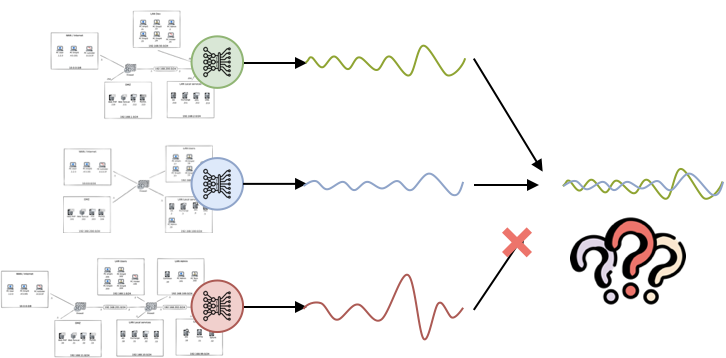
\includegraphics[width=\linewidth]{figures/intro/heterogeneity.png}
    \end{column}

    \begin{column}{.5\textwidth}

      \textcolor<2->{lightgray}{%
      \textbf{Challenge I}: \textit{Too much heterogeneity leads to poor performance\dots}
      }
      \only<1>{%
        \begin{itemize} \small
          \item How to handle different feature sets, data distributions?
          \item How to consider models that are dissimilar because they "contain" relevant knowledge?
        \end{itemize}
      }
      \vspace{1ex}


      \textcolor<1,3>{lightgray}{%
      \textbf{Challenge II}: \textit{Difficult to identify malicious contributions when models are different\dots}
      }
      
      \only<2>{%
        \begin{itemize} \small
          \item Are model "dissimilar" because they are different, or because they are malicious/poisoned?
        \end{itemize}
      }
      \vspace{1ex}
      
      \only<1-2>{\color{lightgray}}
      \textbf{Challenge III}: \textit{No representative dataset of heterogeneous distributed intrusion detection\dots}~\only<3>{\autocite{lavaur_cesar_2022}}
      
      \only<3>{%
      \begin{itemize} \small
          \item Datasets are generated locally, lots of different feature sets, no control over heterogeneity.
        \end{itemize}
      }%
    \end{column}
  \end{columns}

  \only<3>{\fcitefootnote{lavaur_cesar_2022}}
  
\end{frame}


\begin{frame}{Research Questions}
  \begin{enumerate}
    \item What makes applying FL to IDSs specific?
    \item Can FL be used to federate IDSs across heterogeneous data sources?
    \item How does FL handle malicious contributions in a federated IDS?
    \item How can one assess and ensure the trustworthiness of the other participants’ contributions?
  \end{enumerate}
\end{frame}


\begin{frame}[b]{Thesis Summary}
  \centering%
  \foreach \i in {1,...,11} {%
    \includegraphics<\i>[width=1.1\linewidth, center]{./figures/intro/metro/\i.pdf}%
  }
  \includegraphics<12->[width=1.1\linewidth, center]{./figures/intro/metro/12.pdf}%

  \only<13>{
    \tikz[overlay, remember picture,
      shift=(current page.south west),
      x=(current page.south east),
      y=(current page.north west)
    ]{
      % Optional help grid lines
      %\draw[step=.1, opacity=0.3, thick, red] (0,0) grid (1,1);
      
      \node[align=left, anchor=south west] at (.05, .05) {\begin{minipage}{.9\textwidth}
        \tableofcontents
      \end{minipage}};
    }
  }

\end{frame}